\documentclass[10pt, a4paper]{article}

\usepackage[final]{lrec-coling2024} % this is the new style
\usepackage{lipsum}
\usepackage{listings}
\usepackage{booktabs}
\usepackage{hyperref}

\title{MultiWikiQA: A Reading Comprehension Benchmark in 300+ Languages}

\name{Dan Saattrup Smart}

\address{
    Alexandra Institute \\
    dan.smart@alexandra.dk\\
}

\abstract{
    We introduce a new reading comprehension dataset, dubbed MultiWikiQA, which covers
    306 languages. The context data comes from Wikipedia articles, with questions
    generated by an LLM and the answers appearing verbatim in the Wikipedia articles. We
    conduct a crowdsourced human evaluation of the fluency of the generated questions
    across 30 of the languages, providing evidence that the questions are of good
    quality. We evaluate 6 different language models, both decoder and encoder models of
    varying sizes, showing that the benchmark is sufficiently difficult and that there
    is a large performance discrepancy amongst the languages. The dataset and survey
    evaluations are freely available.
}

\begin{document}

\maketitleabstract

\section{Introduction}
Extracting information from documents is one of the primary uses of large language
models (LLMs), especially with the rise of retrieval-augmented generation (RAG) use
cases. Reading comprehension, also known as extractive question answering, is a key
component in such information extraction. At its core, it concerns locating an answer to
the user's query within the provided document.

This relevance of reading comprehension tasks to downstream use cases also increases the
importance of having access to high-quality reading comprehension evaluation datasets
within all languages.

In this work, we generate a reading comprehension dataset for 306 different languages,
based on Wikipedia articles, thus increasing the access to evaluation datasets within
all of these languages. The questions are all generated with an LLM, and we evaluate the
quality of the generated questions within 30+ of the languages through crowdsourcing.
Lastly, we evaluate several language models on all of the languages, mapping out the
performance of these models across a wide variety of languages. Our key contributions
are:

\begin{enumerate}
    \item Release of a multilingual reading comprehension dataset in 306 languages for
      evaluation of  encoder, decoder and encoder-decoder language models.\footnote{The
      dataset can be found at
    \url{https://huggingface.co/datasets/alexandrainst/multi-wiki-qa}.}.
    \item Results and raw data from 156 crowdsourced quality evaluations of the
      LLM-generated questions within the dataset, across 30 languages.\footnote{The raw
      quality evaluation data can be found at [redacted].}.
    \item Evaluations of 6 different language models on 261 languages.
\end{enumerate}


\section{Related Work}
Many reading comprehension datasets have been published in different languages,
including English
\citelanguageresource{rajpurkar-etal-2016-squad,kwiatkowski-etal-2019-natural,joshi-etal-2017-triviaqa},
Polish \citelanguageresource{rybak-etal-2024-polqa}, Korean
\citelanguageresource{jun-etal-2022-korean}, Norwegian
\citelanguageresource{ivanova-etal-2023-norquad,liu-etal-2024-nlebench}, German
\citelanguageresource{moller-etal-2021-germanquad}, French
\citelanguageresource{dhoffschmidt-etal-2020-fquad}, Icelandic
\citelanguageresource{snaebjarnarson-einarsson-2022-natural}, Faroese
\citelanguageresource{simonsen-etal-2025-foqa} and Russian
\citelanguageresource{efimov2020sberquad}. Multilingual reading comprehension datasets
have also been released, covering 7 languages
\citelanguageresource{lewis-etal-2020-mlqa}, 26 languages
\citelanguageresource{longpre-etal-2021-mkqa}, 11 languages
\citelanguageresource{clark-etal-2020-tydi}, and 3 languages
\citelanguageresource{nielsen-2023-scandeval}.

All of these benchmarks only cover a small fraction of the world's written languages,
leaving most of the low-resource languages behind. Belebele
\citelanguageresource{bandarkar-etal-2024-belebele} is a notable exception, which spans
an impressive 122 languages. The multiple-choice format of Belebele is quite different
compared to regular extractive question answering datasets, however. Furthermore, it is
abstractive, contains only 900 samples for each language, and these samples only have
short contexts of approximately 500 characters.


\section{Methodology}
\label{sec:methodology}


\subsection{Dataset Generation}
\label{sec:dataset-generation}

\begin{figure*}[h]
    \centering
    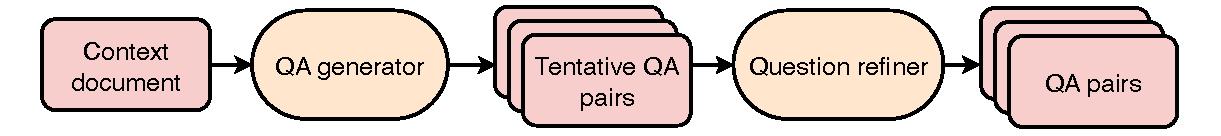
\includegraphics[width=0.9\linewidth]{multi-wiki-qa-process.drawio.pdf}
    \caption{MultiWikiQA dataset generation process.}
    \label{fig:dataset-generation}
\end{figure*}

The dataset generation methodology closely follows the methodology in
\citetlanguageresource{simonsen-etal-2025-foqa}, albeit with minor tweaks and using a
different LLM, which we will describe below - it is also illustrated in
Figure~\ref{fig:dataset-generation}.

From a given document, we start by generating tentative questions and answers with the
LLM using the system and user prompt in Figure~\ref{fig:generation-prompt}. We ask the
model to generate 2-10 different question-answer pairs for each article, both for
efficiency and diversity reasons, since it is more likely to generate new
question-answer pairs when conditioned on the previously generated pairs. We use
structured generation to ensure a valid JSON output.

\begin{figure}
\scriptsize
\begin{verbatim}
SYSTEM:
You are a helpful {language} question answering
dataset generator. The only language you know is
{language}.

USER:
The following is a Wikipedia article in {language}.

<article>
{article}
</article>

Generate 2 to 10 questions about the article,
depending on the length of the article, all
of which answered in the article.

You also have to supply answers to the questions,
and the answers have to appear exactly as written
in the article (including same casing).

The answers should only contain the answers
themselves, and not the surrounding sentence -
keep the answers as short as possible.

The answers have to be different from each other.

All your questions and answers must be in
{language}.

Your answer must be a JSON dictionary with the
key "results", with the value being a list of
dictionaries having keys "question" and "answer".
\end{verbatim}
\caption{The system and user prompt used to generate the tentative questions and answers.}
\label{fig:generation-prompt}
\end{figure}

Next, we filter the generated JSON dictionaries by checking that each question-answer
entry contains the appropriate ``question'' and ``answer'' keys, as well as checking if
the answer appears verbatim in the context document.

We \textit{could} stop at this point, as we now have a set of questions and answers for
the context document. However, other reading comprehension datasets have been criticised
for having questions that used the same wording as the context document, making it too
easy for language models to ``cheat'' by simply word matching
\cite{weissenborn2017making, jia2017adversarial}. In an attempt to prevent this, we
proceed with a separate rephrasing stage, where we prompt the same LLM to rephrase the
question (without the context), using the prompt in Figure~\ref{fig:rephrasing-prompt}.

\begin{figure}
\scriptsize
\begin{verbatim}
The following is a {language} question.

<question>
{question}
</question>

Re-write the question as much as possible,
preserving the meaning, using synonyms,
other phrases, or a different (valid)
word order.

Your question must be in {language}.

Your answer must be a JSON dictionary with the
key "question".
\end{verbatim}
\caption{The prompt used to rephrase the generated tentative questions.}
\label{fig:rephrasing-prompt}
\end{figure}

The resulting set of context-question-answer triples are then collected into a dataset
of the same format as SQuAD~\citelanguageresource{rajpurkar-etal-2016-squad}.


\subsection{Quality Evaluation of LLM-generated Questions}
\label{sec:quality-evaluation}

To evaluate the quality of the LLM-generated questions, we conducted a survey in all the
included languages, and crowdsourced answers from various social media channels. Each
survey contained a random sample of 50 generated questions for the given language, and
prompted the user to rate the fluency of each question as 1, 2, or 3 stars. The precise
preamble that was presented to each user can be seen in
Figure~\ref{fig:survey-preamble}.

\begin{figure*}
    \begin{itshape}
        \small
        Please indicate how natural the following questions are:

        \begin{itemize}
            \item[$\star$] Does not sound natural at all
            \item[$\star\star$] Sounds mostly natural, but there is a particular part of
              the question that looks wrong
            \item[$\star\star\star$] Sounds like a natural question
        \end{itemize}

        Note that ``naturalness'' here is only meaning fluency, so whether the question
        is unanswerable or requires context to be answered does not matter here.
    \end{itshape}
    \caption{The preamble used in all of the surveys.}
    \label{fig:survey-preamble}
\end{figure*}

We used the Microsoft Forms service\footnote{\url{https://forms.cloud.microsoft/}} to
facilitate the individual language surveys, and we self-hosted a simple routing
interface which guided users to the correct language survey - the interface can be seen
in the appendix. As each survey was created manually, we did not create the surveys for
all languages, but instead had the routing interface send us an email if the user
selected a language not currently covered - we then sent an email reply to the user when
the language was included. The routing interface was coded using Vue.js
\cite{you2025vuejs} - the source code can be found in the appendix.

\begin{figure*}[h]
    \centering
    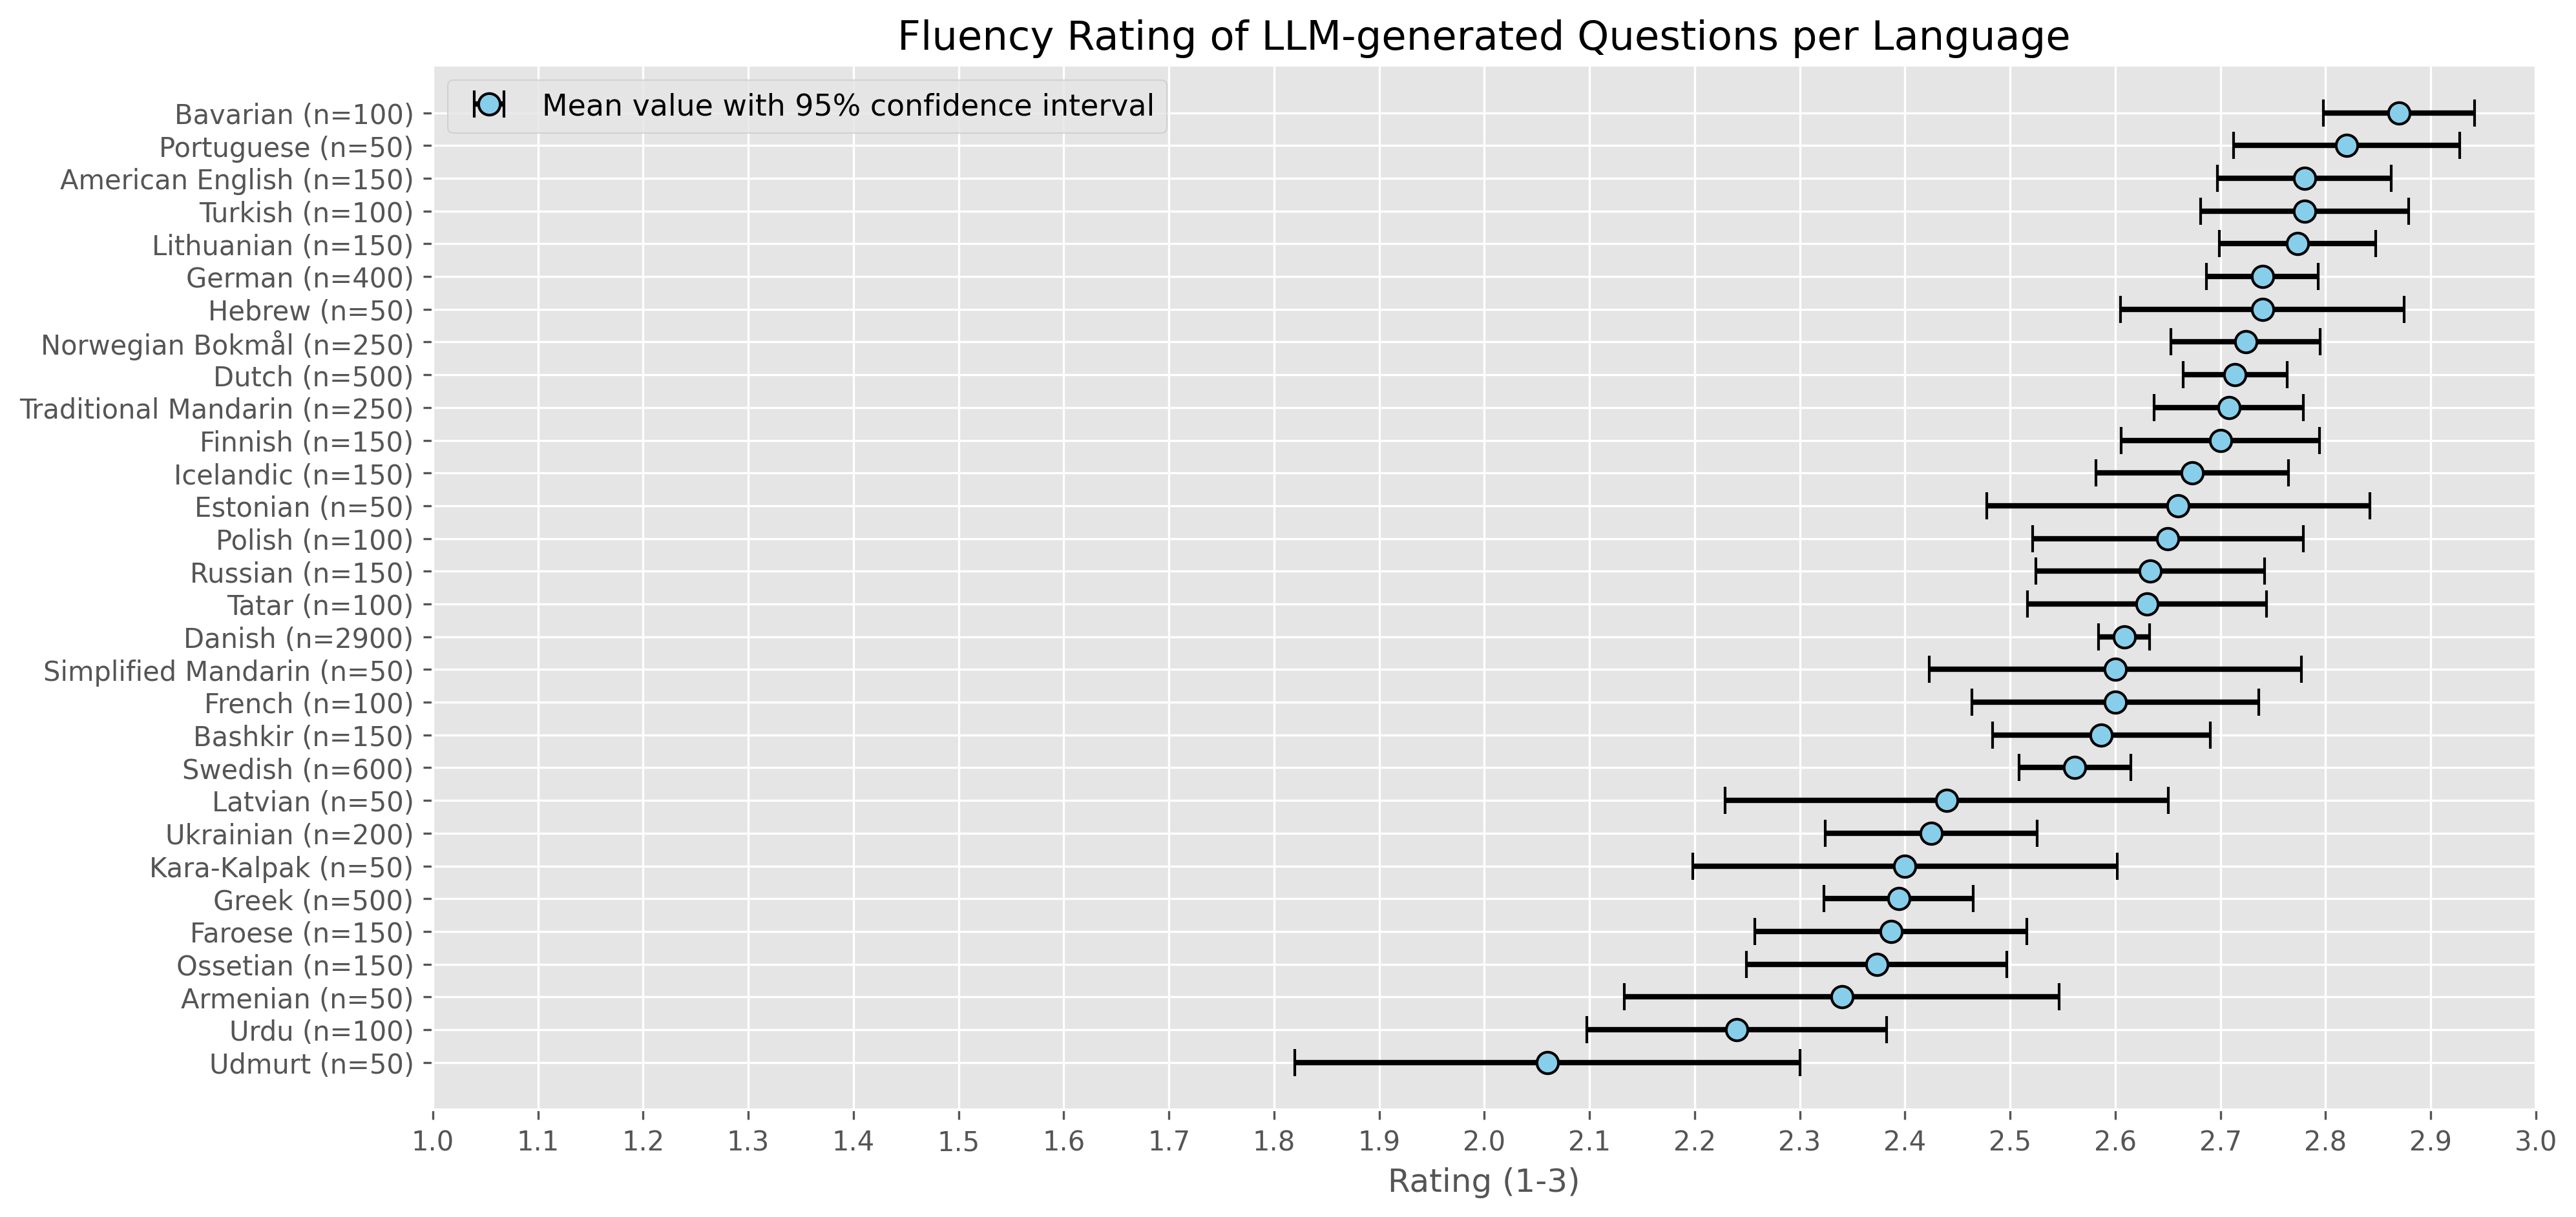
\includegraphics[width=1\linewidth]{fluency-rating-plot.png}
    \caption{Results from the conducted fluency surveys.}
    \label{fig:quality-evaluation-scores}
\end{figure*}

\section{The Dataset}
\label{sec:the-dataset}

We generate the dataset using the methodology in Section~\ref{sec:dataset-generation}.
We use the 20231101 Wikipedia
dump\footnote{\url{https://hf.co/datasets/wikimedia/wikipedia}} and include 315 of the
Wikipedia languages - a full list can be found in the appendix. We include special cases
for Mandarin and Portuguese. We split Mandarin articles into Simplified Mandarin
(``zh-cn'') and Traditional Mandarin (``zh-tw'') using the
HanzIdentifier~\cite{tsroten2024hanzidentifier}, and we split Portuguese articles into
European Portuguese (``pt-pt'') and Brazilian Portuguese (``pt-br'') using the PtVid
classifier~\citelanguageresource{sousa2025enhancing}.

We use the Gemini-1.5-pro model \cite{reid2024gemini} for the question generation with
temperature 1.0 and where we allow 1,000 generated tokens, and we stop generating for a
given language when we reach 5,000 context-question-answer samples, or when we run out
of articles. We ran out of articles for 101 languages - see the appendix for an overview
of these languages.

Using the question evaluation methodology in Section~\ref{sec:quality-evaluation}, we
get 156 survey responses in 30 different languages. The mean quality scores across the
languages, along with the number of survey responses, can be found in
Figure~\ref{fig:quality-evaluation-scores}. We see that the generated questions have a
mean rating above 2.0, corresponding to ``mostly natural'', even for the languages
Bashkir, Kara-Kalpak, Faroese, Ossetian, Udmurt and Icelandic, all having fewer than one
million native speakers.


\section{Evaluations}
\label{sec:evaluations}

\begin{table*}[h]
    \centering
    \small
    \begin{tabular}{lclr}
        \textbf{Model Name} & \textbf{Parameters} & \textbf{Type} & \textbf{Mean F1-score} \\
        \midrule
        Mistral-Small-3.1-24B-Instruct-2503 \cite{mistralsmall2025} & 24B & Instruct Decoder & 55.83\% ± 1.09\% \\
        Mistral-Small-3.1-24B-Base-2503 \cite{mistralsmall2025} & 24B & Base Decoder & 54.71\% ± 1.20\% \\
        Llama-3.1-8B-Instruct \cite{grattafiori2024llama} & 8B & Instruct Decoder & 52.38\% ± 0.91\% \\
        Llama-3.1-8B \cite{grattafiori2024llama} & 8B & Base Decoder & 47.26\% ± 1.22\% \\
        Multilingual-E5-large \cite{wang2024multilingual} & 560M & Encoder & 23.82\% ± 0.65\% \\
        XLM-RoBERTa-large \cite{ruder2019unsupervised} & 561M & Encoder & 20.23\% ± 0.69\% \\
    \end{tabular}
    \caption{Evaluation results on MultiWikiQA in 261 languages}
    \label{tab:evaluated-models}
\end{table*}

\begin{figure*}[h]
    \centering
    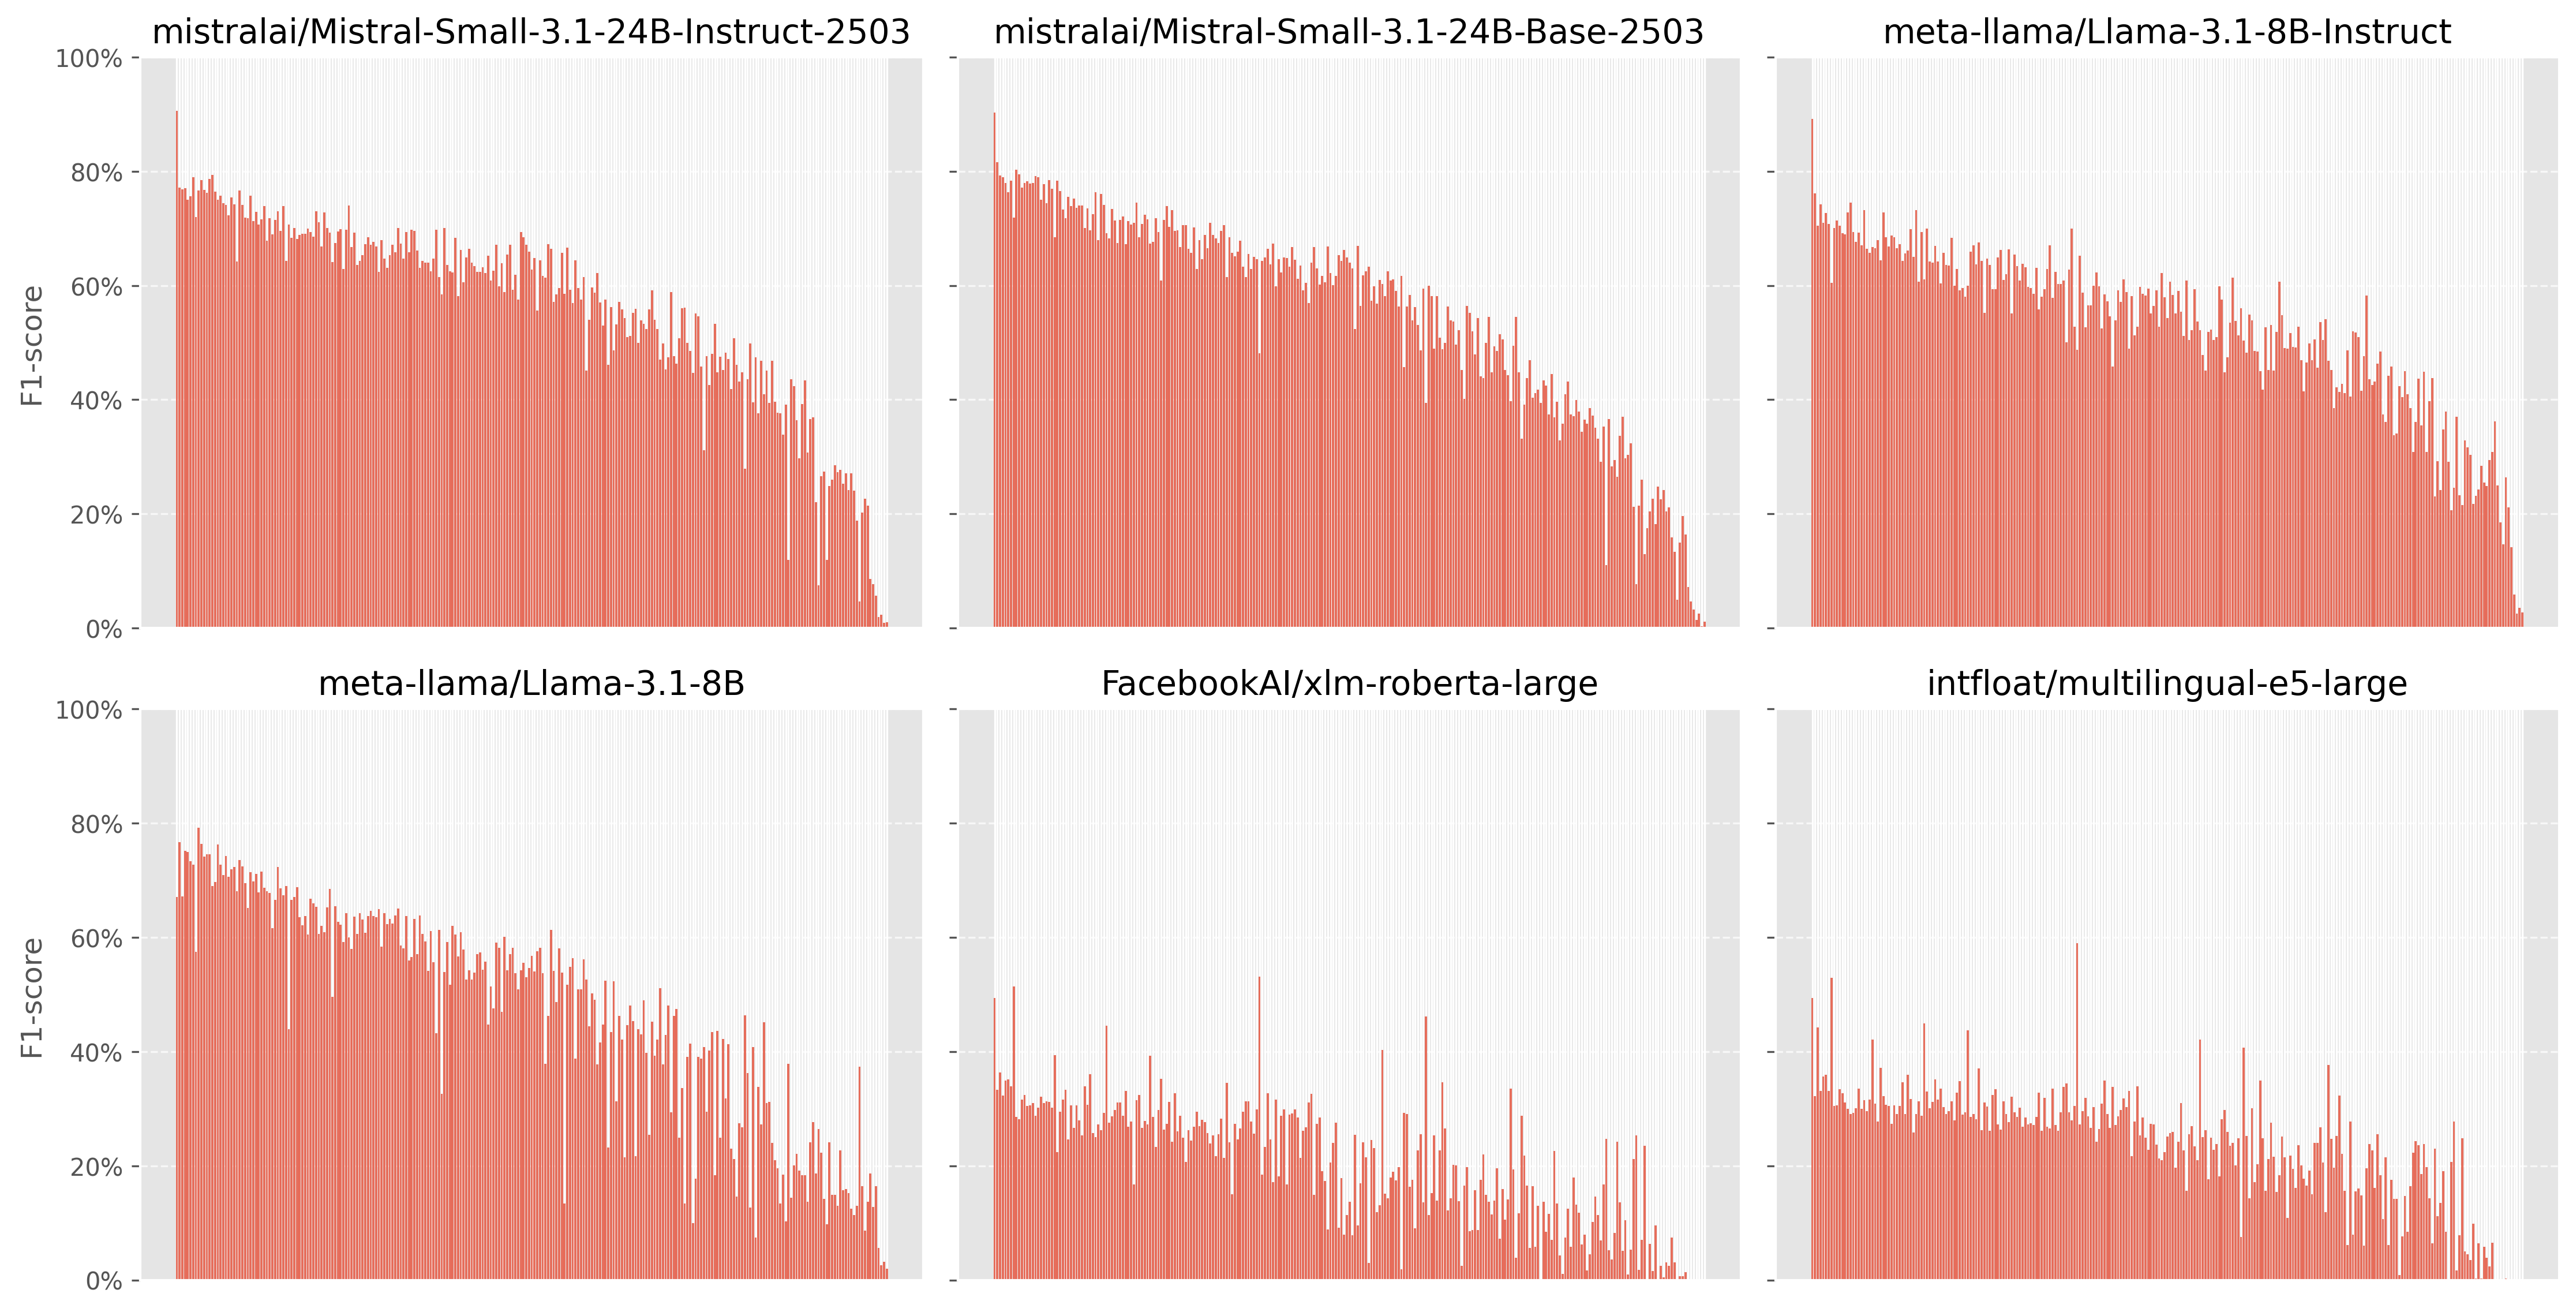
\includegraphics[width=\textwidth]{evaluation-plot.png}
    \caption{F1-score performance of six models across multiple languages, where the
    languages on the x-axis are sorted in descending order based on the mean F1-score
  across all models.}
    \label{fig:evaluation-results}
\end{figure*}

We evaluate a variety of language models on the MultiWikiQA dataset in all the languages
with at least 1,024 samples for training, 32 for validation and 128 for testing. This
was chosen as we are also evaluating encoder models, and 1,024 samples was found in
\citet{nielsen-2023-scandeval} to be enough for the models to adequately fit the data
for several reading comprehension datasets and languages. There were 264 languages
satisfying this criterion.

The evaluation itself was conducted using the EuroEval framework
\cite{nielsen-2023-scandeval,saattrup-nielsen-etal-2025-encoder}. See the list of
evaluated models in Table~\ref{tab:evaluated-models}. The decoder models were evaluated
2-shot, which was preferred over zero-shot evaluation to enable proper evaluation of
base decoder models. The few-shot examples come from the training split. The encoder
models were trained on the training split, with early stopping based on the validation
split, and the final performance reported on the test split.

The results are visualised in Figure~\ref{fig:evaluation-results}, and the full results
can be found in the appendix. From the results, we see that there is a discrepancy in
performance across languages, which is consistent across the three different model
types. We also see that the task is not saturated for any of the languages, and with it
being especially challenging for many of them.


\section{Conclusion}
\label{sec:conclusion}

We have introduced a new reading comprehension dataset in 306 languages, based on
Wikipedia articles, with questions generated by an LLM. We crowdsourced the quality of
the LLM-generated questions for 30 languages, showing that the LLM-generated questions
are of good quality. Lastly, we evaluated 6 models on all of the languages, which showed
that the benchmark is sufficiently difficult across instruction-tuned decoders, base
decoders and encoders, and that there is a large performance discrepancy amongst the
languages.


% Does not count towards the page limit
\section*{Limitations}
\label{sec:limitations}

While we got survey responses in 30 different languages, that still only covers
approximately 10\% of the languages covered in the dataset, so we cannot guarantee that
the conclusions from the surveys generalise to the remaining languages. However, since
the surveys cover a wide spectrum of language families and language resource levels, we
are quite confident in such a generalisation.


% Does not count towards the page limit
\section*{Acknowledgements}
\label{sec:acknowledgements}

This research was funded by the EU Horizon project TrustLLM (grant agreement number
101135671) and the LLM credits used to generate the dataset and evaluate Gemini-2.5-pro
were funded as part of the Google Cloud Research Credits Programme.


\newpage
\nocite{*}
\section{Bibliographical References}\label{sec:reference}

\bibliographystyle{lrec-coling2024-natbib}
\bibliography{bib}

\section{Language Resource References}
\label{lr:ref}
\bibliographystylelanguageresource{lrec-coling2024-natbib}
\bibliographylanguageresource{languageresource}

\newpage
\onecolumn
\appendix

\section{Appendix}

\begin{table*}[h]
    \centering
    \scriptsize
    \begin{tabular}{ccccccccccccc}
        ab & ban & cr & fat & gur & iu & lad & mni & om & ru & ss & tt & yue \\
        ace & bar & crh & ff & guw & ja & lb & mnw & or & rue & st & tum & za \\
        ady & bcl & cs & fi & gv & jam & lbe & mr & os & rw & stq & tw & zea \\
        af & be & csb & fj & ha & jbo & lez & mrj & pa & sa & su & ty & zh-cn \\
        als & bg & cu & fo & hak & ka & lfn & ms & pag & sah & sv & tyv & zh-tw \\
        alt & bi & cv & fon & haw & kaa & lg & mt & pam & sat & sw & udm & zu \\
        am & bjn & cy & fr & he & kab & li & mwl & pap & sc & szl & ug & \\
        ami & blk & da & frp & hi & kbd & lij & my & pcd & scn & szy & uk & \\
        an & bm & dag & frr & hif & kbp & lld & myv & pcm & sco & ta & ur & \\
        ang & bn & de & fur & hr & kcg & lmo & mzn & pdc & sd & tay & uz & \\
        anp & bo & din & fy & hsb & kg & ln & nap & pfl & se & tcy & ve & \\
        ar & bpy & diq & ga & ht & ki & lo & nds & pi & sg & te & vec & \\
        arc & br & dsb & gag & hu & kk & lt & ne & pl & shi & tet & vep & \\
        ary & bs & dty & gan & hy & kl & ltg & new & pms & shn & tg & vi & \\
        arz & bug & dv & gcr & hyw & km & lv & nia & pnb & si & th & vls & \\
        as & bxr & dz & gd & ia & kn & mad & nl & pnt & sk & ti & vo & \\
        ast & ca & ee & gl & id & ko & mai & nn & ps & skr & tk & wa & \\
        atj & cdo & el & glk & ie & koi & mdf & no & pt-br & sl & tl & war & \\
        av & ce & en & gn & ig & krc & mg & nov & pt-pt & sm & tly & wo & \\
        avk & ceb & eo & gom & ik & ks & mhr & nqo & pwn & smn & tn & wuu & \\
        awa & ch & es & gor & ilo & ku & mi & nso & qu & sn & to & xal & \\
        ay & chr & et & got & inh & kv & min & nv & rm & so & tpi & xh & \\
        az & chy & eu & gpe & io & kw & mk & ny & rmy & sq & tr & xmf & \\
        azb & ckb & ext & gu & is & ky & ml & oc & rn & sr & trv & yi & \\
        ba & co & fa & guc & it & la & mn & olo & ro & srn & ts & yo & \\
    \end{tabular}
    \caption{List of all languages in MultiWikiQA.}
    \label{tab:language-overview}
\end{table*}

\begin{table*}[h]
    \centering
    \scriptsize
    \begin{tabular}{cr|cr|cr|cr}
        \textbf{Language} & \textbf{Samples} & \textbf{Language} & \textbf{Samples} & \textbf{Language} & \textbf{Samples} & \textbf{Language} & \textbf{Samples} \\
        \midrule
        lld & 4,745 & tay & 3,049 & guc & 1,558 & cu & 443 \\
        tn & 4,744 & ami & 2,920 & pwn & 1,471 & za & 427 \\
        pcm & 4,623 & nia & 2,804 & mi & 1,419 & ki & 416 \\
        gcr & 4,590 & ny & 2,751 & awa & 1,385 & tpi & 397 \\
        fat & 4,539 & ff & 2,701 & pdc & 1,381 & ti & 385 \\
        om & 4,458 & dz & 2,679 & jam & 1,345 & got & 383 \\
        av & 4,375 & shi & 2,677 & sm & 1,278 & ady & 380 \\
        se & 4,257 & wo & 2,624 & st & 1,270 & lbe & 378 \\
        tum & 4,252 & kbd & 2,585 & ee & 1,223 & ve & 369 \\
        gpe & 4,242 & bpy & 2,561 & kcg & 1,202 & srn & 321 \\
        csb & 4,199 & ln & 2,297 & to & 1,187 & kg & 261 \\
        mrj & 4,194 & ace & 2,210 & tly & 1,108 & arc & 251 \\
        gor & 4,137 & mni & 2,179 & nov & 1,066 & chr & 185 \\
        crh & 4,053 & mad & 2,032 & atj & 1,064 & bi & 149 \\
        gur & 4,042 & jbo & 2,011 & fon & 899 & iu & 148 \\
        dty & 4,029 & hak & 1,945 & nso & 810 & ch & 135 \\
        mdf & 3,957 & haw & 1,903 & pag & 802 & ty & 129 \\
        xh & 3,955 & ss & 1,856 & rn & 763 & bug & 119 \\
        krc & 3,894 & cdo & 1,780 & fj & 745 & sg & 83 \\
        frp & 3,849 & inh & 1,738 & rmy & 722 & pi & 79 \\
        guw & 3,782 & din & 1,716 & gan & 697 & ik & 67 \\
        anp & 3,667 & ltg & 1,636 & nv & 681 & cr & 33 \\
        koi & 3,539 & ab & 1,625 & bm & 663 & chy & 25 \\
        gag & 3,409 & tet & 1,604 & kl & 529 &&\\
        glk & 3,384 & ts & 1,583 & pnt & 529 &&\\
        ang & 3,376 & ks & 1,571 & xal & 464 &&
    \end{tabular}
    \caption{All the languages in MultiWikiQA with fewer than 5,000 samples.}
    \label{tab:num-samples-in-small-subsets}
\end{table*}

\begin{table*}[h]
\centering
\scriptsize
\begin{tabular}{crrrrrr}
\toprule
Language & Mistral Base & Mistral Instruct & Llama Base & Llama Instruct & XLM-RoBERTa & Multi-E5 \\
\midrule
ace & 45.2\% ± 2.2\% & 49.9\% ± 4.1\% & 39.1\% ± 8.2\% & 50.5\% ± 2.5\% & 10.5\% ± 5.6\% & 20.6\% ± 13.9\% \\
af & 78.0\% ± 4.0\% & 76.5\% ± 3.1\% & 69.7\% ± 5.8\% & 74.5\% ± 1.1\% & 30.9\% ± 2.8\% & 29.1\% ± 3.6\% \\
alt & 53.1\% ± 5.7\% & 57.0\% ± 3.7\% & 41.6\% ± 8.6\% & 53.8\% ± 2.5\% & 22.7\% ± 4.1\% & 20.1\% ± 9.5\% \\
am & 21.2\% ± 2.6\% & 22.1\% ± 2.2\% & 18.7\% ± 8.6\% & 20.6\% ± 1.5\% & 21.2\% ± 2.0\% & 20.7\% ± 9.1\% \\
ami & 14.9\% ± 9.1\% & 20.2\% ± 8.0\% & 16.5\% ± 8.1\% & 25.0\% ± 4.7\% & 0.6\% ± 1.4\% & 0.0\% ± 0.0\% \\
an & 71.3\% ± 2.5\% & 69.4\% ± 2.8\% & 66.7\% ± 3.7\% & 63.6\% ± 2.4\% & 26.8\% ± 2.5\% & 29.0\% ± 2.8\% \\
ang & 55.2\% ± 3.3\% & 59.1\% ± 3.1\% & 45.3\% ± 2.8\% & 48.9\% ± 3.0\% & 8.6\% ± 6.4\% & 10.8\% ± 10.1\% \\
anp & 57.3\% ± 4.7\% & 57.2\% ± 4.2\% & 54.2\% ± 3.4\% & 50.5\% ± 3.0\% & 24.6\% ± 4.1\% & 25.5\% ± 4.4\% \\
ar & 68.8\% ± 6.1\% & 65.8\% ± 4.1\% & 63.9\% ± 5.1\% & 59.6\% ± 1.8\% & 25.4\% ± 3.5\% & 27.5\% ± 4.1\% \\
ary & 59.0\% ± 4.5\% & 59.5\% ± 2.8\% & 50.9\% ± 5.0\% & 50.4\% ± 3.0\% & 17.5\% ± 3.4\% & 22.8\% ± 5.1\% \\
arz & 71.9\% ± 6.4\% & 71.9\% ± 5.4\% & 57.5\% ± 5.4\% & 60.4\% ± 5.9\% & 51.5\% ± 2.2\% & 52.9\% ± 2.3\% \\
as & 62.1\% ± 2.5\% & 59.2\% ± 2.9\% & 58.2\% ± 3.2\% & 59.5\% ± 1.7\% & 20.5\% ± 8.8\% & 22.8\% ± 7.7\% \\
ast & 73.3\% ± 2.9\% & 71.9\% ± 3.6\% & 69.5\% ± 4.0\% & 64.4\% ± 2.5\% & 31.6\% ± 6.6\% & 37.1\% ± 3.1\% \\
av & 36.5\% ± 11.3\% & 45.1\% ± 5.0\% & 31.0\% ± 11.8\% & 40.5\% ± 8.6\% & 8.0\% ± 6.5\% & 7.6\% ± 8.4\% \\
avk & 39.7\% ± 6.6\% & 44.7\% ± 3.4\% & 10.0\% ± 7.8\% & 46.8\% ± 2.9\% & 33.5\% ± 3.0\% & 37.7\% ± 2.7\% \\
awa & 67.4\% ± 6.3\% & 68.8\% ± 4.9\% & 63.6\% ± 6.7\% & 67.0\% ± 4.5\% & 31.1\% ± 15.8\% & 35.1\% ± 16.0\% \\
ay & 33.2\% ± 5.3\% & 37.7\% ± 3.7\% & 13.4\% ± 6.4\% & 36.1\% ± 2.8\% & 11.4\% ± 2.7\% & 24.4\% ± 3.5\% \\
az & 71.5\% ± 8.8\% & 69.0\% ± 4.4\% & 62.2\% ± 7.0\% & 64.2\% ± 3.5\% & 31.1\% ± 1.7\% & 31.6\% ± 3.1\% \\
azb & 59.9\% ± 5.1\% & 56.3\% ± 10.0\% & 43.4\% ± 7.6\% & 48.3\% ± 6.0\% & 11.4\% ± 7.5\% & 25.2\% ± 5.3\% \\
ba & 65.8\% ± 6.1\% & 69.5\% ± 4.0\% & 63.2\% ± 3.8\% & 67.0\% ± 2.9\% & 15.0\% ± 6.9\% & 26.6\% ± 5.5\% \\
ban & 60.5\% ± 2.8\% & 65.3\% ± 2.1\% & 44.7\% ± 11.6\% & 61.1\% ± 3.7\% & 26.7\% ± 3.9\% & 31.8\% ± 3.4\% \\
bar & 61.0\% ± 4.3\% & 65.7\% ± 3.5\% & 53.8\% ± 4.6\% & 53.7\% ± 3.2\% & 13.1\% ± 6.4\% & 20.9\% ± 3.1\% \\
bcl & 64.3\% ± 5.4\% & 70.1\% ± 3.5\% & 54.0\% ± 16.0\% & 65.2\% ± 4.6\% & 18.4\% ± 12.5\% & 27.3\% ± 3.3\% \\
be & 65.5\% ± 6.2\% & 62.5\% ± 3.7\% & 61.1\% ± 3.9\% & 50.0\% ± 2.8\% & 31.3\% ± 3.1\% & 34.4\% ± 2.2\% \\
bg & 77.0\% ± 4.2\% & 74.2\% ± 3.7\% & 72.4\% ± 4.2\% & 65.8\% ± 2.8\% & 30.2\% ± 2.1\% & 31.6\% ± 3.1\% \\
bjn & 68.3\% ± 2.2\% & 68.3\% ± 2.6\% & 66.6\% ± 4.2\% & 69.9\% ± 2.3\% & 27.5\% ± 5.3\% & 33.0\% ± 3.5\% \\
blk & 16.4\% ± 5.3\% & 21.4\% ± 2.6\% & 13.7\% ± 2.5\% & 14.7\% ± 2.5\% & 1.4\% ± 3.1\% & 0.0\% ± 0.0\% \\
bn & 62.9\% ± 6.2\% & 64.7\% ± 2.9\% & 55.7\% ± 7.7\% & 62.8\% ± 2.2\% & 27.8\% ± 4.9\% & 29.4\% ± 3.0\% \\
bo & 0.3\% ± 0.4\% & 0.9\% ± 0.8\% & 3.2\% ± 1.6\% & 3.6\% ± 1.8\% & 0.0\% ± 0.1\% & 0.0\% ± 0.0\% \\
bpy & 60.9\% ± 14.7\% & 62.8\% ± 7.0\% & 59.2\% ± 11.5\% & 67.6\% ± 1.5\% & 35.3\% ± 4.1\% & 37.0\% ± 3.9\% \\
br & 68.0\% ± 3.6\% & 67.9\% ± 2.0\% & 58.4\% ± 5.2\% & 63.4\% ± 2.2\% & 27.0\% ± 3.4\% & 28.5\% ± 3.1\% \\
bs & 69.6\% ± 5.4\% & 69.0\% ± 2.9\% & 61.6\% ± 5.2\% & 66.2\% ± 2.2\% & 36.0\% ± 2.6\% & 36.0\% ± 3.2\% \\
bxr & 56.4\% ± 4.6\% & 55.9\% ± 7.1\% & 25.4\% ± 13.1\% & 49.1\% ± 4.5\% & 19.8\% ± 2.7\% & 21.4\% ± 9.5\% \\
ca & 73.9\% ± 4.6\% & 71.3\% ± 4.3\% & 69.8\% ± 3.9\% & 66.8\% ± 2.7\% & 30.6\% ± 4.5\% & 30.5\% ± 3.6\% \\
cdo & 34.4\% ± 6.4\% & 41.0\% ± 3.5\% & 45.2\% ± 6.6\% & 42.3\% ± 10.2\% & 6.2\% ± 8.1\% & 0.8\% ± 3.1\% \\
ce & 49.4\% ± 6.7\% & 55.1\% ± 4.1\% & 17.7\% ± 6.6\% & 45.2\% ± 3.5\% & 19.4\% ± 3.7\% & 24.7\% ± 4.9\% \\
ceb & 69.2\% ± 7.7\% & 70.7\% ± 5.5\% & 43.9\% ± 6.6\% & 61.0\% ± 7.0\% & 44.5\% ± 2.8\% & 44.9\% ± 2.6\% \\
ckb & 35.8\% ± 9.1\% & 27.9\% ± 7.9\% & 46.3\% ± 4.8\% & 48.4\% ± 3.4\% & 1.1\% ± 2.3\% & 18.4\% ± 8.4\% \\
co & 69.6\% ± 6.9\% & 64.3\% ± 4.3\% & 64.3\% ± 8.3\% & 59.3\% ± 5.6\% & 26.0\% ± 11.7\% & 33.5\% ± 4.5\% \\
crh & 63.5\% ± 4.9\% & 63.2\% ± 3.9\% & 54.3\% ± 4.2\% & 59.2\% ± 3.1\% & 21.4\% ± 3.2\% & 28.7\% ± 3.6\% \\
cs & 71.3\% ± 3.7\% & 68.2\% ± 4.1\% & 68.9\% ± 3.3\% & 64.0\% ± 3.1\% & 29.8\% ± 2.4\% & 31.2\% ± 3.6\% \\
csb & 53.9\% ± 7.0\% & 55.2\% ± 3.9\% & 45.4\% ± 6.3\% & 45.1\% ± 5.5\% & 14.3\% ± 7.0\% & 21.1\% ± 3.0\% \\
cv & 37.4\% ± 5.7\% & 41.8\% ± 3.2\% & 23.0\% ± 10.9\% & 58.3\% ± 3.5\% & 11.6\% ± 2.9\% & 19.5\% ± 5.3\% \\
cy & 90.3\% ± 1.9\% & 90.6\% ± 1.3\% & 67.1\% ± 13.0\% & 89.2\% ± 1.9\% & 49.4\% ± 2.6\% & 49.4\% ± 2.2\% \\
da & 78.9\% ± 2.7\% & 77.1\% ± 2.3\% & 75.2\% ± 2.3\% & 74.2\% ± 2.0\% & 32.3\% ± 3.9\% & 33.1\% ± 2.4\% \\
dag & 29.4\% ± 11.3\% & 36.4\% ± 6.0\% & 22.1\% ± 11.5\% & 43.8\% ± 1.6\% & 8.2\% ± 4.5\% & 6.4\% ± 9.4\% \\
de & 80.3\% ± 2.2\% & 76.6\% ± 2.4\% & 79.2\% ± 2.1\% & 70.1\% ± 2.4\% & 28.5\% ± 3.1\% & 30.5\% ± 3.6\% \\
din & 25.9\% ± 8.6\% & 27.4\% ± 7.1\% & 14.2\% ± 6.2\% & 23.3\% ± 5.7\% & 7.0\% ± 11.3\% & 7.9\% ± 12.6\% \\
diq & 43.4\% ± 4.1\% & 48.2\% ± 2.9\% & 31.8\% ± 11.1\% & 41.5\% ± 4.7\% & 13.7\% ± 6.6\% & 14.8\% ± 8.8\% \\
dsb & 61.7\% ± 3.2\% & 61.4\% ± 2.1\% & 37.9\% ± 18.0\% & 55.4\% ± 2.9\% & 24.1\% ± 3.9\% & 31.0\% ± 4.1\% \\
dty & 65.9\% ± 4.0\% & 63.1\% ± 4.4\% & 63.8\% ± 2.5\% & 62.4\% ± 3.1\% & 24.6\% ± 2.0\% & 27.1\% ± 1.6\% \\
dv & 7.2\% ± 6.0\% & 8.5\% ± 6.1\% & 18.7\% ± 8.6\% & 26.3\% ± 4.2\% & 0.1\% ± 0.2\% & 0.2\% ± 0.8\% \\
dz & 1.4\% ± 1.2\% & 1.9\% ± 1.1\% & 5.6\% ± 1.5\% & 5.9\% ± 1.4\% & 0.0\% ± 0.0\% & 0.0\% ± 0.0\% \\
el & 71.6\% ± 4.1\% & 69.2\% ± 2.4\% & 68.5\% ± 4.3\% & 58.0\% ± 3.3\% & 27.3\% ± 3.2\% & 29.3\% ± 3.3\% \\
en & 79.5\% ± 3.9\% & 78.5\% ± 2.7\% & 76.4\% ± 4.4\% & 71.4\% ± 1.7\% & 28.1\% ± 3.6\% & 30.6\% ± 1.9\% \\
eo & 73.6\% ± 5.2\% & 70.6\% ± 4.7\% & 67.9\% ± 5.0\% & 68.5\% ± 2.2\% & 30.6\% ± 3.5\% & 30.6\% ± 3.7\% \\
es & 76.6\% ± 2.6\% & 74.1\% ± 2.1\% & 72.5\% ± 4.7\% & 67.9\% ± 2.7\% & 29.4\% ± 2.6\% & 27.7\% ± 4.4\% \\
et & 73.5\% ± 3.6\% & 71.8\% ± 4.0\% & 67.8\% ± 5.0\% & 65.6\% ± 2.1\% & 30.7\% ± 2.3\% & 29.1\% ± 2.4\% \\
eu & 68.8\% ± 2.9\% & 63.1\% ± 5.2\% & 62.4\% ± 4.1\% & 63.8\% ± 3.4\% & 27.7\% ± 3.9\% & 26.9\% ± 3.3\% \\
ext & 68.2\% ± 4.4\% & 70.0\% ± 4.1\% & 65.1\% ± 4.5\% & 58.6\% ± 4.0\% & 21.7\% ± 4.1\% & 27.2\% ± 2.4\% \\
fa & 68.5\% ± 3.0\% & 66.8\% ± 1.6\% & 62.0\% ± 3.6\% & 62.9\% ± 2.0\% & 32.4\% ± 3.4\% & 32.8\% ± 2.5\% \\
fat & 30.3\% ± 5.0\% & 36.6\% ± 3.5\% & 24.1\% ± 7.7\% & 38.0\% ± 3.5\% & 1.0\% ± 2.4\% & 8.4\% ± 9.2\% \\
ff & 20.4\% ± 8.8\% & 26.0\% ± 5.2\% & 14.9\% ± 4.6\% & 31.6\% ± 2.9\% & 6.3\% ± 5.6\% & 4.5\% ± 8.8\% \\
fi & 69.4\% ± 5.6\% & 69.8\% ± 5.1\% & 62.3\% ± 4.5\% & 63.7\% ± 1.9\% & 29.7\% ± 3.4\% & 28.2\% ± 4.2\% \\
fo & 65.7\% ± 2.0\% & 67.7\% ± 2.9\% & 63.8\% ± 4.1\% & 66.4\% ± 3.3\% & 24.4\% ± 4.8\% & 27.6\% ± 4.8\% \\
\bottomrule
\end{tabular}
\caption{The F1-scores on MultiWikiQA for languages 1-66, sorted alphabetically.}
\label{tab:num-samples-in-small-subsets}
\end{table*}

\begin{table*}[h]
\centering
\scriptsize
\begin{tabular}{crrrrrr}
\toprule
Language & Mistral Base & Mistral Instruct & Llama Base & Llama Instruct & XLM-RoBERTa & Multi-E5 \\
\midrule
fr & 74.1\% ± 4.7\% & 71.6\% ± 1.6\% & 71.5\% ± 3.7\% & 66.5\% ± 1.4\% & 28.0\% ± 2.4\% & 29.1\% ± 4.7\% \\
frp & 62.5\% ± 3.7\% & 59.2\% ± 3.8\% & 54.8\% ± 2.8\% & 45.1\% ± 3.3\% & 14.4\% ± 6.4\% & 26.2\% ± 3.5\% \\
frr & 53.9\% ± 4.2\% & 58.7\% ± 2.9\% & 49.1\% ± 5.1\% & 53.5\% ± 2.5\% & 17.5\% ± 2.5\% & 23.5\% ± 3.0\% \\
fur & 63.0\% ± 5.6\% & 64.8\% ± 4.6\% & 54.0\% ± 9.0\% & 60.7\% ± 2.5\% & 7.8\% ± 4.2\% & 25.8\% ± 2.6\% \\
fy & 68.0\% ± 4.0\% & 69.5\% ± 2.4\% & 68.6\% ± 6.2\% & 73.2\% ± 2.1\% & 27.2\% ± 3.1\% & 29.1\% ± 3.3\% \\
ga & 68.5\% ± 6.0\% & 69.7\% ± 3.3\% & 56.6\% ± 7.7\% & 62.9\% ± 4.9\% & 24.2\% ± 2.7\% & 26.9\% ± 4.3\% \\
gag & 65.2\% ± 2.5\% & 66.1\% ± 1.4\% & 57.1\% ± 6.4\% & 57.8\% ± 1.7\% & 27.3\% ± 4.5\% & 33.5\% ± 3.4\% \\
gcr & 70.7\% ± 5.4\% & 72.8\% ± 3.2\% & 61.0\% ± 4.1\% & 59.2\% ± 6.7\% & 26.7\% ± 2.3\% & 34.8\% ± 2.3\% \\
gd & 70.3\% ± 3.6\% & 66.8\% ± 3.2\% & 58.0\% ± 7.2\% & 64.7\% ± 1.7\% & 31.2\% ± 3.1\% & 30.4\% ± 2.5\% \\
gl & 78.4\% ± 3.9\% & 75.4\% ± 4.7\% & 71.9\% ± 4.5\% & 66.4\% ± 2.5\% & 31.2\% ± 2.5\% & 29.6\% ± 5.1\% \\
glk & 39.9\% ± 9.0\% & 37.6\% ± 6.5\% & 33.9\% ± 5.5\% & 33.8\% ± 3.4\% & 13.2\% ± 4.2\% & 14.2\% ± 12.7\% \\
gn & 21.4\% ± 6.2\% & 26.6\% ± 4.2\% & 22.3\% ± 9.4\% & 37.0\% ± 2.3\% & 1.8\% ± 2.2\% & 1.7\% ± 6.6\% \\
gom & 42.5\% ± 2.8\% & 47.1\% ± 2.6\% & 41.3\% ± 5.3\% & 47.7\% ± 2.5\% & 8.4\% ± 5.1\% & 6.0\% ± 8.6\% \\
gor & 61.4\% ± 3.9\% & 64.0\% ± 2.8\% & 54.1\% ± 5.5\% & 60.9\% ± 3.5\% & 31.3\% ± 2.2\% & 33.8\% ± 2.1\% \\
gpe & 75.0\% ± 2.5\% & 74.5\% ± 1.9\% & 71.0\% ± 3.8\% & 69.3\% ± 2.5\% & 32.1\% ± 2.9\% & 33.5\% ± 3.7\% \\
gu & 61.2\% ± 4.2\% & 62.3\% ± 3.8\% & 57.4\% ± 1.6\% & 53.9\% ± 3.4\% & 28.5\% ± 3.1\% & 27.2\% ± 5.0\% \\
guc & 19.6\% ± 6.2\% & 22.7\% ± 5.0\% & 8.7\% ± 3.6\% & 18.5\% ± 3.1\% & 0.6\% ± 2.3\% & 0.0\% ± 0.1\% \\
gur & 37.2\% ± 5.7\% & 39.7\% ± 3.6\% & 20.9\% ± 9.6\% & 38.5\% ± 1.8\% & 10.1\% ± 6.1\% & 16.4\% ± 7.0\% \\
guw & 17.5\% ± 9.2\% & 24.8\% ± 4.8\% & 24.1\% ± 5.0\% & 32.8\% ± 2.5\% & 0.2\% ± 0.7\% & 5.0\% ± 8.0\% \\
gv & 52.2\% ± 4.5\% & 53.8\% ± 2.5\% & 43.0\% ± 8.6\% & 51.8\% ± 2.0\% & 13.8\% ± 3.3\% & 15.4\% ± 7.5\% \\
ha & 52.4\% ± 4.9\% & 55.6\% ± 2.6\% & 57.6\% ± 3.4\% & 58.3\% ± 2.3\% & 25.4\% ± 4.1\% & 25.9\% ± 5.2\% \\
hak & 37.4\% ± 8.6\% & 39.5\% ± 7.5\% & 40.8\% ± 10.6\% & 44.2\% ± 6.8\% & 5.9\% ± 7.5\% & 6.2\% ± 9.8\% \\
haw & 38.5\% ± 11.3\% & 46.8\% ± 7.8\% & 24.0\% ± 8.7\% & 40.9\% ± 6.4\% & 4.5\% ± 6.7\% & 8.4\% ± 12.7\% \\
he & 73.2\% ± 3.8\% & 69.2\% ± 3.1\% & 63.7\% ± 3.9\% & 63.6\% ± 2.8\% & 24.2\% ± 3.4\% & 26.2\% ± 4.1\% \\
hi & 67.6\% ± 5.3\% & 67.4\% ± 3.5\% & 65.5\% ± 8.0\% & 65.9\% ± 2.1\% & 28.5\% ± 1.5\% & 28.5\% ± 2.6\% \\
hif & 70.6\% ± 4.3\% & 67.2\% ± 2.0\% & 60.8\% ± 3.9\% & 66.3\% ± 2.8\% & 25.0\% ± 3.5\% & 26.3\% ± 3.6\% \\
hr & 64.6\% ± 5.0\% & 64.7\% ± 2.5\% & 64.3\% ± 2.8\% & 60.9\% ± 2.4\% & 28.1\% ± 2.7\% & 30.2\% ± 2.6\% \\
hsb & 60.2\% ± 4.1\% & 63.9\% ± 2.4\% & 47.0\% ± 11.7\% & 52.8\% ± 3.5\% & 28.5\% ± 4.7\% & 33.9\% ± 3.9\% \\
ht & 79.3\% ± 4.0\% & 76.9\% ± 3.2\% & 67.1\% ± 2.9\% & 70.5\% ± 2.3\% & 36.3\% ± 1.8\% & 44.2\% ± 1.4\% \\
hu & 66.6\% ± 7.5\% & 65.3\% ± 5.9\% & 63.2\% ± 5.7\% & 63.2\% ± 3.8\% & 25.8\% ± 3.0\% & 28.4\% ± 1.7\% \\
hy & 64.0\% ± 10.4\% & 62.6\% ± 6.9\% & 47.6\% ± 5.1\% & 48.9\% ± 3.2\% & 32.6\% ± 2.0\% & 33.1\% ± 2.6\% \\
hyw & 56.3\% ± 7.9\% & 54.0\% ± 8.0\% & 44.5\% ± 2.6\% & 44.8\% ± 3.0\% & 29.0\% ± 2.8\% & 29.8\% ± 2.0\% \\
ia & 72.1\% ± 2.9\% & 69.1\% ± 3.4\% & 63.8\% ± 2.3\% & 60.4\% ± 2.7\% & 28.7\% ± 2.3\% & 33.6\% ± 2.5\% \\
id & 77.9\% ± 3.9\% & 75.0\% ± 3.5\% & 75.0\% ± 3.4\% & 71.0\% ± 2.5\% & 34.9\% ± 3.0\% & 35.7\% ± 3.2\% \\
ie & 76.3\% ± 4.3\% & 75.6\% ± 4.4\% & 73.4\% ± 3.3\% & 72.7\% ± 2.5\% & 35.1\% ± 1.8\% & 36.0\% ± 2.8\% \\
ig & 45.2\% ± 5.6\% & 53.3\% ± 3.4\% & 49.0\% ± 6.9\% & 60.7\% ± 2.1\% & 2.5\% ± 2.7\% & 18.4\% ± 12.5\% \\
ilo & 56.2\% ± 4.8\% & 62.2\% ± 2.4\% & 37.8\% ± 16.2\% & 61.4\% ± 2.6\% & 9.0\% ± 6.0\% & 24.0\% ± 5.9\% \\
inh & 33.7\% ± 6.9\% & 39.2\% ± 6.1\% & 18.3\% ± 7.3\% & 29.3\% ± 4.3\% & 13.6\% ± 8.6\% & 11.2\% ± 14.5\% \\
io & 68.5\% ± 5.2\% & 64.2\% ± 5.0\% & 68.1\% ± 3.8\% & 66.7\% ± 2.3\% & 39.3\% ± 3.4\% & 42.2\% ± 1.8\% \\
is & 70.7\% ± 2.8\% & 68.6\% ± 2.5\% & 66.0\% ± 4.1\% & 63.5\% ± 1.6\% & 27.7\% ± 2.0\% & 29.5\% ± 3.5\% \\
it & 76.3\% ± 3.5\% & 73.0\% ± 1.9\% & 72.3\% ± 4.4\% & 65.0\% ± 1.5\% & 25.0\% ± 3.2\% & 25.8\% ± 3.1\% \\
ja & 50.0\% ± 3.4\% & 47.4\% ± 4.3\% & 48.1\% ± 4.3\% & 41.5\% ± 3.5\% & 14.9\% ± 3.6\% & 17.8\% ± 3.6\% \\
jam & 54.5\% ± 6.2\% & 54.6\% ± 5.4\% & 39.1\% ± 4.9\% & 38.5\% ± 6.8\% & 3.9\% ± 6.4\% & 19.7\% ± 6.7\% \\
ka & 66.4\% ± 7.0\% & 62.4\% ± 3.9\% & 51.7\% ± 2.2\% & 52.7\% ± 1.9\% & 32.7\% ± 3.8\% & 31.9\% ± 2.1\% \\
kaa & 58.1\% ± 5.9\% & 57.1\% ± 4.6\% & 46.2\% ± 5.2\% & 48.5\% ± 3.1\% & 13.9\% ± 4.9\% & 17.1\% ± 8.7\% \\
kab & 22.7\% ± 7.3\% & 28.5\% ± 6.3\% & 14.9\% ± 4.4\% & 30.3\% ± 2.4\% & 1.5\% ± 2.3\% & 3.5\% ± 6.4\% \\
kbd & 32.4\% ± 5.8\% & 36.9\% ± 5.0\% & 27.7\% ± 7.3\% & 29.1\% ± 3.6\% & 5.3\% ± 7.5\% & 0.0\% ± 0.0\% \\
kbp & 13.4\% ± 11.7\% & 18.9\% ± 13.3\% & 13.0\% ± 7.1\% & 30.8\% ± 3.7\% & 3.0\% ± 4.6\% & 6.6\% ± 12.0\% \\
kk & 69.6\% ± 8.1\% & 63.6\% ± 9.0\% & 60.6\% ± 7.0\% & 59.4\% ± 5.5\% & 32.7\% ± 3.0\% & 32.4\% ± 5.5\% \\
km & 7.7\% ± 5.0\% & 7.4\% ± 3.8\% & 26.4\% ± 8.3\% & 24.6\% ± 3.4\% & 25.3\% ± 3.4\% & 27.7\% ± 3.6\% \\
kn & 66.7\% ± 2.8\% & 63.4\% ± 1.9\% & 53.8\% ± 3.3\% & 54.6\% ± 2.1\% & 29.2\% ± 6.6\% & 26.6\% ± 8.5\% \\
ko & 60.8\% ± 5.5\% & 57.0\% ± 4.3\% & 56.4\% ± 5.1\% & 51.8\% ± 2.7\% & 18.0\% ± 12.1\% & 17.6\% ± 10.5\% \\
koi & 37.1\% ± 9.8\% & 47.5\% ± 3.0\% & 7.5\% ± 6.3\% & 45.8\% ± 2.2\% & 17.9\% ± 8.8\% & 17.6\% ± 13.1\% \\
krc & 59.9\% ± 3.5\% & 58.4\% ± 3.9\% & 48.7\% ± 3.3\% & 52.2\% ± 2.0\% & 23.1\% ± 8.5\% & 26.9\% ± 11.6\% \\
ks & 44.8\% ± 4.4\% & 45.8\% ± 3.5\% & 38.7\% ± 5.6\% & 42.2\% ± 5.9\% & 11.7\% ± 7.9\% & 25.2\% ± 11.7\% \\
ku & 62.5\% ± 5.0\% & 67.2\% ± 2.6\% & 46.2\% ± 5.3\% & 51.2\% ± 2.8\% & 21.5\% ± 8.5\% & 22.7\% ± 4.7\% \\
kv & 48.5\% ± 6.7\% & 50.7\% ± 6.9\% & 24.9\% ± 14.0\% & 50.6\% ± 3.4\% & 19.5\% ± 5.7\% & 24.0\% ± 5.2\% \\
kw & 41.7\% ± 11.3\% & 47.5\% ± 5.1\% & 24.9\% ± 12.1\% & 51.8\% ± 3.5\% & 13.0\% ± 4.0\% & 15.5\% ± 4.8\% \\
ky & 59.8\% ± 9.9\% & 58.2\% ± 6.0\% & 56.7\% ± 2.9\% & 60.0\% ± 3.2\% & 31.6\% ± 2.1\% & 30.2\% ± 2.2\% \\
la & 67.5\% ± 5.8\% & 67.3\% ± 4.7\% & 58.6\% ± 4.4\% & 63.1\% ± 2.6\% & 25.5\% ± 2.3\% & 28.6\% ± 3.7\% \\
lad & 70.2\% ± 2.6\% & 66.8\% ± 2.8\% & 63.5\% ± 3.0\% & 55.1\% ± 2.8\% & 26.8\% ± 3.5\% & 32.1\% ± 3.2\% \\
lb & 71.0\% ± 3.8\% & 73.0\% ± 6.3\% & 65.4\% ± 4.0\% & 68.3\% ± 2.6\% & 16.7\% ± 4.5\% & 31.3\% ± 4.1\% \\
lez & 48.0\% ± 5.0\% & 52.4\% ± 4.0\% & 42.1\% ± 4.2\% & 49.3\% ± 2.5\% & 15.7\% ± 6.4\% & 19.4\% ± 7.1\% \\
lfn & 71.0\% ± 2.4\% & 67.1\% ± 1.8\% & 62.4\% ± 3.7\% & 59.8\% ± 2.2\% & 23.9\% ± 4.2\% & 27.3\% ± 4.9\% \\
lg & 28.4\% ± 11.8\% & 42.4\% ± 6.4\% & 20.0\% ± 7.1\% & 39.7\% ± 1.6\% & 3.6\% ± 4.7\% & 14.3\% ± 9.0\% \\
\bottomrule
\end{tabular}
\caption{The F1-scores on MultiWikiQA for languages 66-131, sorted alphabetically.}
\label{tab:num-samples-in-small-subsets}
\end{table*}

\begin{table*}[h]
\centering
\scriptsize
\begin{tabular}{crrrrrr}
\toprule
Language & Mistral Base & Mistral Instruct & Llama Base & Llama Instruct & XLM-RoBERTa & Multi-E5 \\
\midrule
li & 64.6\% ± 3.3\% & 66.2\% ± 2.9\% & 60.9\% ± 2.9\% & 62.3\% ± 1.8\% & 18.2\% ± 8.7\% & 24.3\% ± 4.5\% \\
lij & 66.9\% ± 2.6\% & 64.4\% ± 3.9\% & 58.2\% ± 3.1\% & 55.1\% ± 1.8\% & 9.6\% ± 7.5\% & 19.7\% ± 6.4\% \\
lld & 51.9\% ± 9.8\% & 54.0\% ± 1.9\% & 39.3\% ± 14.9\% & 51.7\% ± 3.3\% & 8.8\% ± 6.8\% & 21.8\% ± 9.5\% \\
lmo & 64.9\% ± 4.2\% & 66.0\% ± 4.7\% & 54.6\% ± 11.3\% & 57.9\% ± 2.3\% & 11.4\% ± 6.2\% & 22.4\% ± 4.4\% \\
ln & 32.9\% ± 19.6\% & 44.8\% ± 12.0\% & 26.8\% ± 12.0\% & 46.3\% ± 2.9\% & 4.3\% ± 3.6\% & 25.5\% ± 7.2\% \\
lo & 13.0\% ± 5.7\% & 11.9\% ± 3.9\% & 9.8\% ± 7.7\% & 21.5\% ± 2.5\% & 23.5\% ± 4.0\% & 24.8\% ± 8.1\% \\
lt & 70.1\% ± 5.2\% & 67.9\% ± 4.7\% & 68.1\% ± 3.0\% & 64.3\% ± 2.6\% & 33.9\% ± 2.1\% & 34.6\% ± 4.4\% \\
ltg & 61.1\% ± 5.4\% & 64.4\% ± 3.9\% & 38.7\% ± 6.8\% & 52.2\% ± 6.6\% & 19.0\% ± 13.0\% & 24.9\% ± 13.2\% \\
lv & 67.3\% ± 5.9\% & 70.0\% ± 4.1\% & 60.6\% ± 5.7\% & 65.7\% ± 1.6\% & 33.1\% ± 2.5\% & 30.3\% ± 13.0\% \\
mad & 56.8\% ± 5.4\% & 59.5\% ± 3.5\% & 58.1\% ± 4.6\% & 59.4\% ± 2.9\% & 11.9\% ± 8.8\% & 23.4\% ± 5.6\% \\
mai & 63.3\% ± 5.8\% & 64.0\% ± 4.4\% & 59.3\% ± 3.7\% & 60.2\% ± 3.0\% & 29.4\% ± 2.6\% & 29.4\% ± 5.1\% \\
mdf & 36.9\% ± 10.0\% & 46.1\% ± 3.1\% & 14.6\% ± 6.8\% & 42.6\% ± 2.3\% & 22.6\% ± 2.7\% & 22.7\% ± 3.0\% \\
mg & 48.8\% ± 7.1\% & 54.3\% ± 4.0\% & 21.5\% ± 9.5\% & 45.0\% ± 2.5\% & 34.7\% ± 14.0\% & 35.0\% ± 16.3\% \\
mhr & 48.9\% ± 5.7\% & 53.2\% ± 3.6\% & 31.3\% ± 10.5\% & 53.9\% ± 3.6\% & 25.3\% ± 6.1\% & 30.1\% ± 4.9\% \\
mi & 64.8\% ± 3.9\% & 66.4\% ± 3.9\% & 54.3\% ± 11.4\% & 58.4\% ± 5.3\% & 16.7\% ± 11.0\% & 34.9\% ± 6.2\% \\
min & 66.5\% ± 3.3\% & 67.1\% ± 3.0\% & 64.7\% ± 4.1\% & 62.0\% ± 2.1\% & 26.2\% ± 2.8\% & 29.1\% ± 3.0\% \\
mk & 74.4\% ± 3.9\% & 72.3\% ± 2.1\% & 70.6\% ± 3.7\% & 73.2\% ± 1.8\% & 31.3\% ± 3.1\% & 31.5\% ± 2.1\% \\
ml & 64.9\% ± 1.5\% & 64.9\% ± 2.8\% & 52.6\% ± 1.9\% & 52.5\% ± 2.4\% & 29.9\% ± 3.5\% & 30.8\% ± 2.6\% \\
mn & 63.3\% ± 6.0\% & 64.0\% ± 4.5\% & 52.6\% ± 11.2\% & 57.2\% ± 2.4\% & 28.9\% ± 2.4\% & 29.1\% ± 2.3\% \\
mni & 1.1\% ± 0.7\% & 1.0\% ± 0.6\% & 2.0\% ± 0.7\% & 2.7\% ± 1.5\% & 0.0\% ± 0.0\% & 0.0\% ± 0.0\% \\
mnw & 4.7\% ± 4.1\% & 7.7\% ± 3.5\% & 12.8\% ± 4.5\% & 21.2\% ± 4.3\% & 0.1\% ± 0.3\% & 0.0\% ± 0.0\% \\
mr & 71.8\% ± 3.8\% & 71.8\% ± 1.8\% & 65.2\% ± 6.1\% & 72.8\% ± 1.8\% & 33.3\% ± 3.3\% & 32.2\% ± 5.8\% \\
mrj & 44.0\% ± 9.7\% & 49.9\% ± 5.7\% & 37.8\% ± 10.1\% & 52.8\% ± 2.6\% & 17.5\% ± 3.3\% & 23.6\% ± 9.2\% \\
ms & 81.6\% ± 2.2\% & 77.1\% ± 2.2\% & 76.7\% ± 1.6\% & 76.1\% ± 2.3\% & 33.3\% ± 3.5\% & 32.3\% ± 3.1\% \\
mt & 61.7\% ± 4.7\% & 61.5\% ± 3.6\% & 56.1\% ± 3.6\% & 59.9\% ± 1.7\% & 1.9\% ± 2.8\% & 18.2\% ± 9.3\% \\
mwl & 76.1\% ± 4.3\% & 73.9\% ± 1.9\% & 67.4\% ± 7.6\% & 60.6\% ± 2.4\% & 26.3\% ± 4.4\% & 31.3\% ± 5.8\% \\
my & 26.4\% ± 7.8\% & 29.8\% ± 5.8\% & 19.2\% ± 5.9\% & 23.0\% ± 5.1\% & 24.2\% ± 5.6\% & 23.0\% ± 4.4\% \\
myv & 39.7\% ± 4.0\% & 43.2\% ± 3.2\% & 27.4\% ± 8.3\% & 43.2\% ± 2.5\% & 13.4\% ± 5.9\% & 16.2\% ± 10.7\% \\
mzn & 56.3\% ± 7.2\% & 57.5\% ± 5.4\% & 50.9\% ± 6.3\% & 51.0\% ± 3.5\% & 19.7\% ± 3.2\% & 23.8\% ± 2.1\% \\
nap & 66.8\% ± 3.4\% & 67.1\% ± 3.3\% & 57.1\% ± 4.2\% & 58.3\% ± 2.1\% & 8.9\% ± 8.9\% & 24.9\% ± 5.0\% \\
nds & 72.5\% ± 3.1\% & 71.5\% ± 3.4\% & 66.6\% ± 4.2\% & 69.9\% ± 2.4\% & 25.8\% ± 5.4\% & 31.7\% ± 4.4\% \\
ne & 62.8\% ± 4.7\% & 62.4\% ± 3.5\% & 65.0\% ± 2.8\% & 65.4\% ± 2.4\% & 29.5\% ± 1.3\% & 29.3\% ± 3.0\% \\
new & 39.4\% ± 15.3\% & 46.1\% ± 12.1\% & 23.2\% ± 16.7\% & 50.4\% ± 10.0\% & 46.1\% ± 3.9\% & 40.7\% ± 17.5\% \\
nia & 24.2\% ± 6.9\% & 27.1\% ± 5.1\% & 15.9\% ± 5.8\% & 28.4\% ± 2.3\% & 0.5\% ± 1.5\% & 0.2\% ± 0.9\% \\
nl & 78.3\% ± 4.0\% & 78.7\% ± 2.8\% & 74.6\% ± 4.2\% & 69.0\% ± 1.7\% & 30.4\% ± 2.8\% & 31.1\% ± 3.3\% \\
nn & 77.9\% ± 4.5\% & 76.2\% ± 2.8\% & 74.6\% ± 4.7\% & 69.2\% ± 1.7\% & 32.4\% ± 3.2\% & 32.7\% ± 3.4\% \\
no & 77.1\% ± 4.3\% & 76.7\% ± 2.3\% & 74.2\% ± 3.7\% & 70.4\% ± 2.7\% & 31.6\% ± 2.8\% & 33.4\% ± 2.2\% \\
nqo & 2.5\% ± 0.9\% & 2.3\% ± 0.9\% & 2.6\% ± 0.4\% & 2.5\% ± 0.6\% & 0.0\% ± 0.1\% & 0.0\% ± 0.1\% \\
ny & 51.5\% ± 4.1\% & 56.1\% ± 3.6\% & 33.6\% ± 7.4\% & 45.6\% ± 2.4\% & 7.2\% ± 5.5\% & 24.1\% ± 4.7\% \\
oc & 65.0\% ± 4.8\% & 63.6\% ± 2.2\% & 59.2\% ± 4.0\% & 58.7\% ± 1.3\% & 23.3\% ± 2.6\% & 29.5\% ± 1.8\% \\
olo & 60.0\% ± 4.4\% & 61.9\% ± 3.1\% & 53.8\% ± 4.0\% & 55.1\% ± 3.0\% & 24.0\% ± 2.9\% & 27.4\% ± 3.6\% \\
om & 18.2\% ± 8.2\% & 27.3\% ± 4.9\% & 13.0\% ± 6.6\% & 21.7\% ± 9.1\% & 9.6\% ± 5.5\% & 9.9\% ± 9.3\% \\
or & 33.2\% ± 1.8\% & 31.1\% ± 2.1\% & 40.8\% ± 5.4\% & 41.3\% ± 1.6\% & 28.8\% ± 3.2\% & 32.3\% ± 3.7\% \\
os & 44.3\% ± 6.2\% & 48.6\% ± 4.3\% & 41.4\% ± 6.4\% & 54.1\% ± 3.6\% & 14.1\% ± 4.2\% & 11.8\% ± 13.3\% \\
pa & 73.9\% ± 3.4\% & 74.0\% ± 2.6\% & 60.0\% ± 4.6\% & 55.2\% ± 5.2\% & 27.4\% ± 4.2\% & 31.1\% ± 2.9\% \\
pam & 40.1\% ± 15.2\% & 52.3\% ± 2.4\% & 39.8\% ± 9.7\% & 54.8\% ± 2.3\% & 16.5\% ± 3.2\% & 25.1\% ± 2.2\% \\
pap & 74.0\% ± 2.0\% & 73.9\% ± 2.4\% & 68.7\% ± 4.9\% & 67.2\% ± 3.7\% & 25.4\% ± 3.3\% & 30.5\% ± 2.6\% \\
pcd & 70.6\% ± 5.3\% & 68.5\% ± 4.3\% & 63.7\% ± 4.9\% & 60.9\% ± 3.0\% & 20.7\% ± 8.5\% & 31.3\% ± 2.2\% \\
pcm & 78.3\% ± 1.7\% & 76.6\% ± 2.0\% & 73.6\% ± 2.2\% & 66.5\% ± 1.9\% & 22.4\% ± 9.9\% & 30.9\% ± 2.1\% \\
pdc & 58.2\% ± 7.8\% & 66.7\% ± 7.0\% & 51.7\% ± 5.0\% & 47.8\% ± 4.5\% & 15.1\% ± 9.6\% & 25.0\% ± 9.3\% \\
pfl & 64.3\% ± 2.0\% & 68.4\% ± 1.7\% & 55.6\% ± 4.3\% & 52.8\% ± 4.8\% & 17.8\% ± 4.2\% & 21.3\% ± 5.4\% \\
pl & 69.6\% ± 5.5\% & 64.7\% ± 3.8\% & 58.1\% ± 6.7\% & 55.8\% ± 2.6\% & 28.2\% ± 5.5\% & 32.8\% ± 4.3\% \\
pms & 66.7\% ± 3.4\% & 67.2\% ± 4.0\% & 59.1\% ± 5.1\% & 58.1\% ± 2.9\% & 15.0\% ± 5.6\% & 21.7\% ± 7.2\% \\
pnb & 61.6\% ± 3.4\% & 58.9\% ± 1.8\% & 60.1\% ± 2.4\% & 59.7\% ± 2.1\% & 19.1\% ± 5.3\% & 25.3\% ± 9.0\% \\
ps & 49.9\% ± 6.7\% & 50.9\% ± 4.2\% & 44.7\% ± 2.9\% & 41.8\% ± 4.1\% & 26.5\% ± 5.2\% & 24.8\% ± 5.8\% \\
pt-br & 79.2\% ± 5.3\% & 75.0\% ± 6.2\% & 76.3\% ± 3.9\% & 69.3\% ± 2.6\% & 28.7\% ± 3.2\% & 29.3\% ± 4.4\% \\
pt-pt & 77.7\% ± 1.5\% & 74.1\% ± 2.3\% & 74.2\% ± 3.9\% & 67.0\% ± 1.6\% & 31.0\% ± 3.5\% & 30.0\% ± 6.3\% \\
pwn & 20.4\% ± 7.4\% & 24.2\% ± 5.5\% & 15.2\% ± 5.5\% & 25.4\% ± 4.7\% & 3.1\% ± 5.2\% & 5.8\% ± 9.2\% \\
qu & 50.5\% ± 12.1\% & 56.1\% ± 3.2\% & 13.4\% ± 7.9\% & 53.6\% ± 2.3\% & 16.0\% ± 3.6\% & 26.7\% ± 4.6\% \\
rm & 60.5\% ± 4.0\% & 65.4\% ± 3.1\% & 54.2\% ± 2.5\% & 58.6\% ± 2.8\% & 17.4\% ± 2.1\% & 28.5\% ± 3.4\% \\
ro & 75.2\% ± 2.2\% & 72.9\% ± 2.6\% & 71.1\% ± 3.4\% & 68.8\% ± 2.7\% & 26.6\% ± 2.8\% & 27.4\% ± 5.0\% \\
ru & 63.0\% ± 6.1\% & 59.9\% ± 5.2\% & 58.2\% ± 5.2\% & 51.3\% ± 4.3\% & 27.3\% ± 1.8\% & 27.8\% ± 2.3\% \\
rue & 64.5\% ± 2.4\% & 62.4\% ± 2.5\% & 57.1\% ± 3.6\% & 45.8\% ± 2.3\% & 29.9\% ± 3.7\% & 33.8\% ± 3.6\% \\
rw & 44.5\% ± 3.4\% & 50.7\% ± 3.2\% & 21.1\% ± 8.0\% & 43.6\% ± 1.8\% & 7.0\% ± 3.6\% & 23.9\% ± 4.7\% \\
sa & 50.9\% ± 4.8\% & 55.8\% ± 4.5\% & 42.1\% ± 13.9\% & 48.5\% ± 2.6\% & 22.7\% ± 1.9\% & 20.3\% ± 9.1\% \\
\bottomrule
\end{tabular}
\caption{The F1-scores on MultiWikiQA for languages 131-196, sorted alphabetically.}
\label{tab:num-samples-in-small-subsets}
\end{table*}

\begin{table*}[h]
\centering
\scriptsize
\begin{tabular}{crrrrrr}
\toprule
Language & Mistral Base & Mistral Instruct & Llama Base & Llama Instruct & XLM-RoBERTa & Multi-E5 \\
\midrule
sah & 41.1\% ± 4.4\% & 44.8\% ± 3.7\% & 43.6\% ± 5.8\% & 52.0\% ± 1.9\% & 5.8\% ± 6.2\% & 7.9\% ± 12.2\% \\
sat & 5.0\% ± 3.1\% & 4.7\% ± 3.3\% & 37.3\% ± 4.1\% & 36.2\% ± 1.6\% & 0.0\% ± 0.0\% & 0.0\% ± 0.0\% \\
sc & 64.0\% ± 3.7\% & 62.8\% ± 3.2\% & 56.8\% ± 5.8\% & 54.3\% ± 2.5\% & 13.7\% ± 6.2\% & 25.1\% ± 4.4\% \\
scn & 65.4\% ± 6.2\% & 69.3\% ± 3.7\% & 54.2\% ± 5.7\% & 59.2\% ± 3.4\% & 9.2\% ± 8.2\% & 23.7\% ± 4.7\% \\
sco & 75.6\% ± 3.6\% & 75.7\% ± 2.9\% & 71.4\% ± 5.1\% & 68.4\% ± 3.1\% & 24.7\% ± 2.9\% & 30.7\% ± 4.1\% \\
sd & 45.7\% ± 5.2\% & 45.1\% ± 5.6\% & 52.6\% ± 7.3\% & 57.6\% ± 4.5\% & 29.3\% ± 4.4\% & 28.1\% ± 1.6\% \\
se & 54.5\% ± 6.6\% & 58.9\% ± 5.0\% & 29.4\% ± 10.3\% & 46.5\% ± 5.2\% & 13.7\% ± 2.7\% & 16.5\% ± 5.1\% \\
shi & 24.8\% ± 4.3\% & 27.7\% ± 2.3\% & 22.7\% ± 4.6\% & 23.2\% ± 2.8\% & 0.1\% ± 0.2\% & 0.2\% ± 0.6\% \\
shn & 3.2\% ± 3.6\% & 5.7\% ± 3.7\% & 16.4\% ± 2.9\% & 14.2\% ± 3.1\% & 0.2\% ± 0.4\% & 0.0\% ± 0.0\% \\
si & 11.0\% ± 7.7\% & 11.9\% ± 3.7\% & 37.9\% ± 4.9\% & 44.9\% ± 2.3\% & 24.7\% ± 2.1\% & 23.8\% ± 2.5\% \\
sk & 72.4\% ± 4.1\% & 70.1\% ± 3.2\% & 65.3\% ± 4.8\% & 59.5\% ± 1.8\% & 27.9\% ± 4.6\% & 28.9\% ± 3.5\% \\
skr & 49.3\% ± 2.8\% & 46.3\% ± 4.1\% & 47.5\% ± 2.6\% & 46.9\% ± 2.3\% & 13.9\% ± 6.8\% & 15.0\% ± 7.6\% \\
sl & 71.5\% ± 7.4\% & 69.8\% ± 4.7\% & 64.3\% ± 5.3\% & 64.3\% ± 2.7\% & 26.3\% ± 5.1\% & 26.2\% ± 6.4\% \\
smn & 53.7\% ± 2.7\% & 56.0\% ± 2.7\% & 21.7\% ± 13.4\% & 53.1\% ± 2.8\% & 20.1\% ± 5.2\% & 27.5\% ± 4.1\% \\
sn & 43.1\% ± 5.9\% & 49.9\% ± 5.0\% & 12.7\% ± 6.1\% & 36.1\% ± 4.9\% & 12.5\% ± 11.1\% & 21.5\% ± 10.0\% \\
so & 39.1\% ± 11.1\% & 47.7\% ± 3.0\% & 29.5\% ± 3.7\% & 42.7\% ± 3.7\% & 21.8\% ± 2.3\% & 22.1\% ± 2.0\% \\
sq & 67.8\% ± 5.5\% & 64.3\% ± 3.9\% & 60.6\% ± 5.0\% & 60.3\% ± 1.4\% & 26.5\% ± 2.0\% & 26.1\% ± 5.8\% \\
sr & 62.3\% ± 6.6\% & 60.6\% ± 4.3\% & 57.9\% ± 6.2\% & 59.9\% ± 5.3\% & 28.7\% ± 2.2\% & 26.4\% ± 11.6\% \\
ss & 36.6\% ± 6.8\% & 43.6\% ± 6.3\% & 14.4\% ± 7.8\% & 30.8\% ± 3.8\% & 5.2\% ± 5.5\% & 19.7\% ± 5.3\% \\
stq & 56.4\% ± 4.3\% & 61.6\% ± 2.8\% & 53.8\% ± 5.0\% & 59.0\% ± 2.0\% & 17.0\% ± 4.6\% & 24.2\% ± 3.3\% \\
su & 65.0\% ± 4.1\% & 69.7\% ± 1.7\% & 43.3\% ± 13.6\% & 70.0\% ± 2.9\% & 25.7\% ± 3.5\% & 28.0\% ± 2.5\% \\
sv & 78.3\% ± 2.4\% & 79.0\% ± 1.8\% & 72.8\% ± 5.1\% & 70.8\% ± 1.6\% & 33.9\% ± 2.8\% & 33.1\% ± 2.9\% \\
sw & 77.8\% ± 3.4\% & 79.4\% ± 1.1\% & 69.0\% ± 2.2\% & 72.8\% ± 1.4\% & 30.6\% ± 2.7\% & 30.0\% ± 4.2\% \\
szl & 58.3\% ± 9.0\% & 59.7\% ± 6.8\% & 50.2\% ± 9.9\% & 47.4\% ± 7.2\% & 16.3\% ± 7.6\% & 26.0\% ± 3.1\% \\
szy & 15.8\% ± 6.1\% & 24.0\% ± 3.2\% & 11.4\% ± 5.2\% & 29.4\% ± 3.3\% & 7.4\% ± 2.4\% & 2.4\% ± 5.6\% \\
ta & 61.4\% ± 6.3\% & 65.8\% ± 4.2\% & 56.0\% ± 5.3\% & 59.4\% ± 1.9\% & 34.6\% ± 2.9\% & 31.9\% ± 3.1\% \\
tay & 35.3\% ± 5.4\% & 39.1\% ± 4.6\% & 10.3\% ± 5.6\% & 35.5\% ± 3.1\% & 16.7\% ± 4.9\% & 18.6\% ± 7.1\% \\
tcy & 41.0\% ± 2.6\% & 43.5\% ± 2.8\% & 36.2\% ± 5.0\% & 37.4\% ± 3.1\% & 7.4\% ± 6.2\% & 10.6\% ± 9.5\% \\
te & 74.5\% ± 1.4\% & 71.1\% ± 2.0\% & 60.7\% ± 3.2\% & 60.0\% ± 2.2\% & 31.5\% ± 1.7\% & 27.9\% ± 12.7\% \\
tet & 66.3\% ± 4.5\% & 67.1\% ± 2.5\% & 53.1\% ± 4.9\% & 62.2\% ± 3.5\% & 8.0\% ± 6.6\% & 21.0\% ± 18.2\% \\
tg & 63.3\% ± 3.1\% & 66.4\% ± 2.1\% & 61.3\% ± 3.8\% & 60.9\% ± 2.2\% & 3.0\% ± 2.3\% & 15.6\% ± 12.3\% \\
th & 63.7\% ± 2.6\% & 62.3\% ± 2.2\% & 62.1\% ± 3.4\% & 56.5\% ± 3.7\% & 24.6\% ± 11.3\% & 28.7\% ± 2.0\% \\
tk & 59.4\% ± 2.8\% & 57.5\% ± 3.1\% & 52.5\% ± 3.2\% & 56.1\% ± 1.8\% & 13.6\% ± 3.4\% & 7.5\% ± 10.1\% \\
tl & 73.4\% ± 3.4\% & 70.0\% ± 2.6\% & 67.1\% ± 4.7\% & 64.3\% ± 2.7\% & 28.6\% ± 2.9\% & 30.1\% ± 2.7\% \\
tn & 29.1\% ± 12.9\% & 33.8\% ± 14.9\% & 18.5\% ± 15.6\% & 43.7\% ± 5.0\% & 6.9\% ± 5.7\% & 23.6\% ± 4.5\% \\
tr & 74.1\% ± 3.0\% & 64.3\% ± 2.0\% & 69.0\% ± 5.5\% & 69.4\% ± 1.3\% & 29.3\% ± 4.0\% & 28.7\% ± 4.6\% \\
trv & 35.1\% ± 2.7\% & 37.7\% ± 2.5\% & 19.6\% ± 6.4\% & 30.8\% ± 5.2\% & 14.6\% ± 7.1\% & 22.3\% ± 4.8\% \\
ts & 29.7\% ± 9.2\% & 30.8\% ± 8.9\% & 13.7\% ± 5.9\% & 34.8\% ± 7.6\% & 10.4\% ± 10.9\% & 19.1\% ± 20.5\% \\
tt & 67.4\% ± 21.8\% & 64.1\% ± 20.5\% & 49.6\% ± 16.6\% & 60.0\% ± 3.8\% & 39.3\% ± 2.8\% & 43.7\% ± 4.6\% \\
tum & 40.4\% ± 11.5\% & 53.3\% ± 7.2\% & 18.3\% ± 8.7\% & 40.5\% ± 7.2\% & 16.5\% ± 4.0\% & 27.7\% ± 12.0\% \\
tw & 35.8\% ± 3.2\% & 39.4\% ± 2.4\% & 31.2\% ± 8.9\% & 45.0\% ± 2.9\% & 1.7\% ± 1.7\% & 14.7\% ± 12.1\% \\
tyv & 44.8\% ± 3.8\% & 47.7\% ± 2.6\% & 46.2\% ± 5.7\% & 49.9\% ± 2.5\% & 11.5\% ± 5.3\% & 19.1\% ± 9.1\% \\
udm & 57.0\% ± 6.1\% & 60.9\% ± 3.4\% & 51.4\% ± 9.0\% & 58.9\% ± 3.2\% & 31.1\% ± 3.0\% & 30.2\% ± 4.6\% \\
ug & 43.8\% ± 11.5\% & 45.3\% ± 4.4\% & 42.9\% ± 5.1\% & 46.9\% ± 3.7\% & 22.0\% ± 4.4\% & 20.1\% ± 9.2\% \\
uk & 64.6\% ± 6.0\% & 61.5\% ± 2.9\% & 61.4\% ± 7.1\% & 52.8\% ± 2.1\% & 29.9\% ± 2.4\% & 30.5\% ± 3.3\% \\
ur & 66.7\% ± 6.7\% & 65.4\% ± 4.7\% & 63.2\% ± 6.7\% & 64.9\% ± 3.5\% & 28.8\% ± 2.0\% & 27.3\% ± 3.9\% \\
uz & 61.7\% ± 6.8\% & 57.5\% ± 2.8\% & 50.9\% ± 3.1\% & 56.4\% ± 2.0\% & 27.5\% ± 2.4\% & 27.2\% ± 2.5\% \\
vec & 67.3\% ± 4.0\% & 68.4\% ± 3.0\% & 60.6\% ± 4.0\% & 56.5\% ± 4.2\% & 17.2\% ± 4.6\% & 26.6\% ± 5.7\% \\
vep & 48.6\% ± 3.1\% & 53.0\% ± 1.4\% & 44.7\% ± 3.0\% & 51.3\% ± 2.1\% & 25.6\% ± 2.9\% & 24.8\% ± 11.7\% \\
vi & 78.9\% ± 5.5\% & 75.8\% ± 4.5\% & 72.8\% ± 7.3\% & 67.7\% ± 3.7\% & 30.1\% ± 3.2\% & 30.1\% ± 2.7\% \\
vls & 70.6\% ± 4.5\% & 69.3\% ± 3.5\% & 63.8\% ± 4.6\% & 58.0\% ± 2.9\% & 21.4\% ± 3.1\% & 26.1\% ± 11.4\% \\
vo & 60.2\% ± 5.4\% & 58.5\% ± 5.6\% & 13.4\% ± 10.9\% & 52.1\% ± 7.5\% & 40.3\% ± 3.9\% & 42.1\% ± 2.6\% \\
wa & 46.9\% ± 3.6\% & 48.1\% ± 2.4\% & 43.4\% ± 4.2\% & 48.7\% ± 2.3\% & 5.6\% ± 4.4\% & 6.1\% ± 9.6\% \\
war & 48.1\% ± 16.6\% & 58.5\% ± 8.9\% & 32.6\% ± 11.7\% & 48.8\% ± 5.3\% & 53.1\% ± 2.7\% & 59.0\% ± 4.1\% \\
wo & 22.6\% ± 6.8\% & 25.3\% ± 5.0\% & 15.7\% ± 4.8\% & 24.3\% ± 3.6\% & 2.5\% ± 3.8\% & 6.4\% ± 10.2\% \\
wuu & 43.8\% ± 6.9\% & 42.6\% ± 4.7\% & 40.2\% ± 4.0\% & 41.1\% ± 1.8\% & 16.5\% ± 2.9\% & 15.6\% ± 7.8\% \\
xh & 37.0\% ± 6.3\% & 43.4\% ± 5.3\% & 18.3\% ± 6.7\% & 24.1\% ± 3.9\% & 5.1\% ± 3.2\% & 13.5\% ± 6.2\% \\
xmf & 49.7\% ± 2.6\% & 50.0\% ± 3.0\% & 43.9\% ± 2.0\% & 45.1\% ± 1.1\% & 20.1\% ± 3.1\% & 21.5\% ± 9.8\% \\
yi & 59.2\% ± 6.8\% & 62.2\% ± 2.7\% & 55.8\% ± 5.1\% & 57.1\% ± 2.9\% & 26.1\% ± 3.4\% & 29.7\% ± 4.3\% \\
yo & 39.4\% ± 5.0\% & 45.2\% ± 7.3\% & 42.2\% ± 4.8\% & 51.0\% ± 3.3\% & 0.1\% ± 0.3\% & 16.0\% ± 8.6\% \\
yue & 56.3\% ± 3.5\% & 51.2\% ± 2.6\% & 48.1\% ± 5.1\% & 52.7\% ± 2.3\% & 12.2\% ± 8.4\% & 15.6\% ± 6.9\% \\
zea & 71.8\% ± 2.5\% & 69.5\% ± 2.9\% & 62.8\% ± 5.6\% & 67.0\% ± 2.3\% & 23.3\% ± 3.4\% & 29.1\% ± 3.6\% \\
zh-cn & 54.3\% ± 2.9\% & 47.0\% ± 2.8\% & 51.1\% ± 4.9\% & 49.2\% ± 3.6\% & 8.8\% ± 11.3\% & 16.1\% ± 8.7\% \\
zh-tw & 58.1\% ± 4.3\% & 48.7\% ± 2.7\% & 52.4\% ± 3.0\% & 54.9\% ± 2.4\% & 15.3\% ± 7.1\% & 14.3\% ± 11.1\% \\
zu & 37.9\% ± 5.0\% & 46.8\% ± 4.8\% & 27.2\% ± 4.8\% & 34.0\% ± 2.4\% & 11.8\% ± 6.6\% & 14.2\% ± 11.3\% \\
\bottomrule
\end{tabular}
\caption{The F1-scores on MultiWikiQA for languages 196-261, sorted alphabetically.}
\label{tab:num-samples-in-small-subsets}
\end{table*}


\begin{figure*}
    \centering
    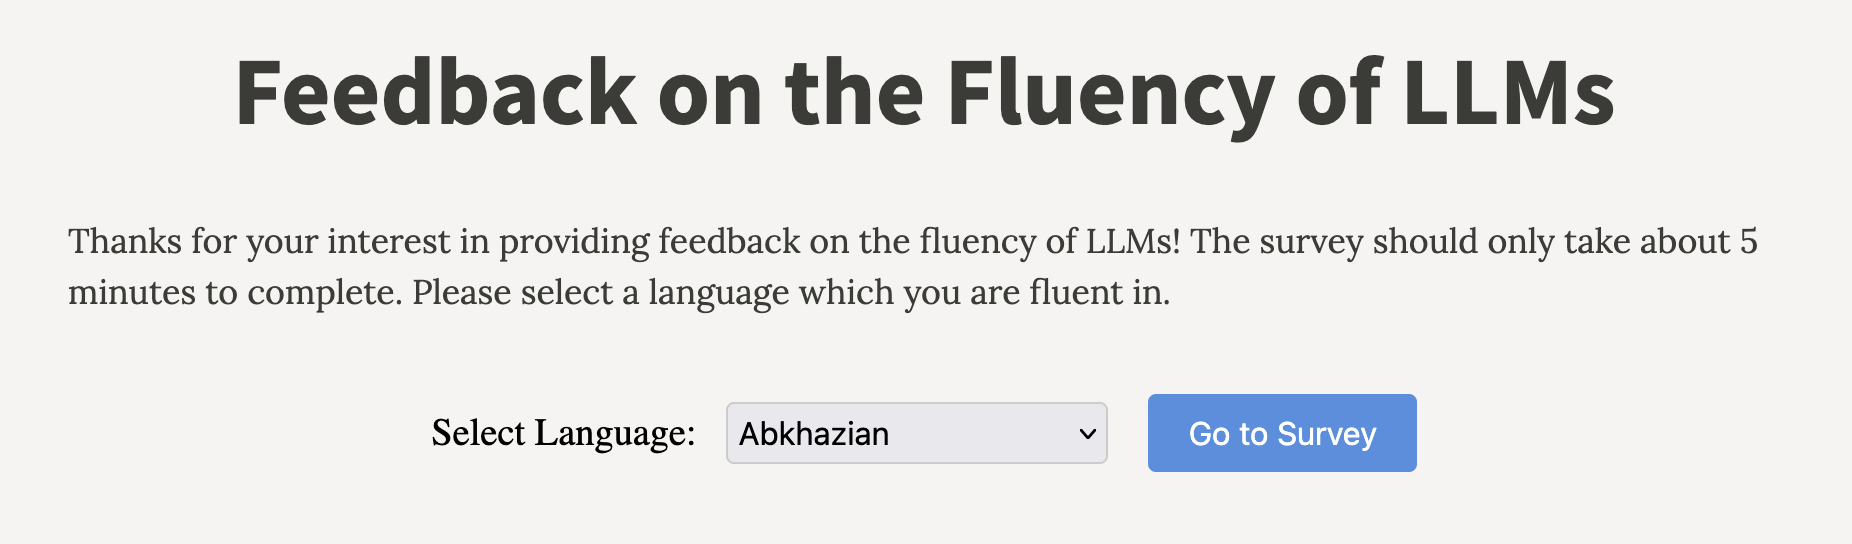
\includegraphics[width=1.0\linewidth]{routing-interface.png}
    \caption{The survey routing interface.}
    \label{fig:routing-interface}
\end{figure*}

\begin{figure*}[h]
\scriptsize
\centering
\begin{tabular}{c}
\begin{lstlisting}
<script lang="ts" setup>
const languageToSurveyUrl: Record<string, string> = {
  Abkhazian: "https://forms.cloud.microsoft/e/pdmAKbsRk1",
  Acehnese: "",
  (...)
};

function goToSurvey() {
  const selectElement = document.getElementById(
    "language-select",
  ) as HTMLSelectElement;
  const selectedLanguage = selectElement.value;
  const surveyUrl = languageToSurveyUrl[selectedLanguage];
  if (surveyUrl) {
    window.open(surveyUrl, "_blank");
  } else {
    window.open(
      "mailto:[redacted]@[redacted].[redacted]?" +
        "subject=Fluency%20Survey%20Language%20Support - " +
        selectedLanguage +
        "&" +
        "body=I would like to request support for " +
        selectedLanguage +
        " in the fluency survey. Thanks!",
      "_blank",
    );
  }
}
</script>
<template>
  <h1 class="centered">Feedback on the Fluency of LLMs</h1>
  <p class="centered-box serif-text">
    Thanks for your interest in providing feedback on the fluency of LLMs! The
    survey should only take about 5 minutes to complete. Please select a
    language which you are fluent in.
  </p>

  <br />
  <br />

  <div class="centered">
    <label for="language-select" class="language-label"
      >Select Language:
    </label>
    <select id="language-select" class="dropdown">
      <option
        v-for="language in Object.keys(languageToSurveyUrl)"
        v-bind:key="language"
        :value="language"
      >
        {{ language }}
      </option>
    </select>
    <button class="button" @click="goToSurvey">Go to Survey</button>
  </div>
</template>
<style scoped>
h1 {
  font-size: 3rem;
}
.centered {
  text-align: center;
}
.language-label {
  font-size: 1.2rem;
  margin-right: 10px;
}
.dropdown {
  font-size: 1rem;
  padding: 5px;
  margin-right: 20px;
  border: 1px solid #ccc;
  border-radius: 4px;
}
.button {
  font-size: 1rem;
  padding: 10px 20px;
  color: white;
  background-color: #4a90e2;
  border: none;
  border-radius: 4px;
  cursor: pointer;
}
.button:hover {
  background-color: #357abd;
}
</style>
\end{lstlisting}
\end{tabular}
\caption{The source code for the Vue.js survey routing interface component}
\end{figure*}

\end{document}
